Having discussed the various steps in the LEP process, and the nuance required in modeling, we now turn to a more-practical discussion, regarding direct measurement of pitch-angle scattering due to wave-particle interactions. 

The following chapter represents somewhat of a detour from the preceding chapters. In the first few years of my time at Stanford, I worked on a hardware design for a CubeSat-based measurement platform, designed specifically for the study of these interactions. The project, named the VLF Wave-Particle Precipitation Mapper, or VPM, formed a nexus of several research projects within the Stanford VLF group -- numerical modeling, fault-tolerant chip design, and embedded systems development -- and granted our small team of graduate students and research scientists design experience for a space-based mission.

In order to quantify the relative effect of waves on particle distributions, one needs to measure two quantities: The incident wave, in the form of electric and magnetic fields, and the pitch angles of the particles impinging on the satellite. VPM samples the wave by measuring two of the six wave components -- one E and one B measurement, perpendicular to each other -- and the distribution of pitch angle distribution using two electron spectrometers, oriented such that one samples only particles within the loss cone, and the other only trapped particles.

The VPM team was led by Dr. Robert Marshall and Dr. Ivan Linscott; the bulk of the hardware design was done by Jeff Chang and Steven Ingram. Additional software and hardware design was done by Christopher Young, Jordan Lenoach, and Alex Cousland. My primary contribution was the design and implementation of all the onboard firmware and digital signal processing. Design of the electron pitch-angle spectrometer system was contracted to a group at Lockheed Martin, as we lacked the facilities or the expertise to work with energetic particles.

%One disclaimer to those embarking on a CubeSat design, or other space-based system: It seems to me that the final design of a project is dictated as much by well-intentioned engineering practices as it is by the constraints levied on the project. 
Our design was dictated by two primary constraints: 1) Design with the ability to exchange all commercial-grade components with space-rated components, and in an effort to reduce the risk of catastrophic computer failures, 2) that the system include no embedded firmware or programs stored in volatile memory. These constraints left a marked imprint on our final design. In a sense, we designed for a conventional satellite mission, with the notable exception that our instrument was small.

Were I to do this project again, from scratch, I would strongly advocate following the CubeSat ethos: Sacrifice bulletproof reliability in exchange for rapid design and prototyping, and affordability of flight components. CubeSat missions generally fly in low-earth orbit ($\sim 400$ km altitude), and have mission lifetimes on the order of a few years, at maximum, due to atmospheric drag. While the idea of a fully radiation-tolerant design is alluring, it is hard to justify the price increase in parts (often $\sim$1000 x greater), and the difficulty in designing for them, for a short-duration, academic mission.

This chapter was mostly written shortly after delivery of the initial VPM prototype, in January, 2015. Both VPM and DSX were delayed several years afterward; as of writing, VPM has been picked up by a new group at AFRL, and is slated to launch in January, 2019.

\section{VPM Mission Overview}
The VLF Wave and Particle Precipitation Mapper (VPM) is a 3U CubeSat designed to measure wave activity and relativistic electrons in the Earth's radiation belts from low-Earth orbit (LEO). The VPM payload consists of an electric field dipole antenna and a magnetic field search coil to measure waves in the VLF frequency band from 100 Hz to 30 kHz; and two electron detectors, designed to measure electron energies from 100 keV to 1 MeV. In addition to single-spacecraft scientific goals outlined below, VPM is a companion to the Wave-Induced Precipitation of Electron Radiation (WIPER) experiment on the Demonstration and Science Experiments (DSX) mission \citep{Schoenberg2006, Spanjers2006}, a small spacecraft designed to investigate the Earth's radiation belts using active probing techniques. Both spacecraft are scheduled to be launched in 2019.

VPM will study the Earth's radiation belts from Low-Earth Orbit (LEO). The radiation belts are comprised of relativistic electrons from hundreds of keV to tens of MeV, and protons from tens to hundreds of MeV. These energetic particles can be highly damaging to spacecraft and to astronauts \citep[e.g.][]{Barth2003}, and comprise a vital component of space weather which affects satellite navigation and communication \citep{Bothmer:2007}. The distribution and evolution of radiation belt populations are controlled by geomagnetic activity and by wave activity in the plasmasphere. Radiation belt particles can be scattered in energy and pitch angle by magnetic reconfiguration, and by wave activity, which can include Alfvenic, electrostatic and electromagnetic waves. Waves can energize these particles, or cause them to precipitate and be lost to the Earth's upper atmosphere. The extent to which wave activity of different sources controls radiation belt distributions and lifetimes is still under considerable investigation. For example, the current Van Allen Probes (VAP) mission, launched in 2012, is particularly investigating the processes that accelerate and transport radiation belt electrons; radiation belt loss mechanisms; and the effects of geomagnetic storms on the radiation belts \citep{Spence2014}. %, Lanzerotti:2013 

Specific science goals of the VPM mission are:

\begin{enumerate}
\item Improve climatology models of plasmaspheric hiss
\item Conduct conjunction experiments with the DSX mission and WIPER instrument
	\begin{enumerate}
	\item Measure the Antenna Radiation Pattern of the WIPER VLF transmitter known as the TNT (Transmitter, Narrow-band receiver, and Tuners)
	\item Measure the Radiation Efficiency of the TNT
	\item Estimate the efficiency of Wave-Particle interactions using WIPER-injected waves
	\end{enumerate}
\item Improve understanding of the effects of Lightning in the near-Earth space environment
	\begin{enumerate}
	\item Improve climatology models of lightning and whistler activity
	\item Estimate the efficiency of lightning whistler-induced wave-particle interactions
	\end{enumerate}
\item Improve understanding of the effects of VLF transmitters in the near-Earth space environment
	\begin{enumerate}
	\item Measure the efficiency of propagation in the earth-ionosphere waveguide and leakage into the ionosphere and magnetosphere
	\item Estimate the efficiency of VLF transmitter whistler-induced wave-particle interactions
	\end{enumerate}
\item Measure the trans-ionospheric absorption of lightning-generated sferics and whistlers
\item Measure VLF wave propagation characteristics in the near-Earth space environment
\item Validate models of wave-particle interactions
\end{enumerate}


Here we present the design of the VPM payload instrumentation and data processing, with an emphasis on the VLF wave instrumentation and data processing unit. The VPM payload is unique in a number of ways: i) four science instruments have been collocated in 1.5U of payload space; ii) all data processing is handled in firmware, reducing the power requirements and eliminating any software from the payload; and iii) data products are delivered with maximum flexibility thanks to the unique implementation of processing methods. These unique aspects of VPM will be discussed in sections to follow.


\begin{figure}[t]
\begin{center}
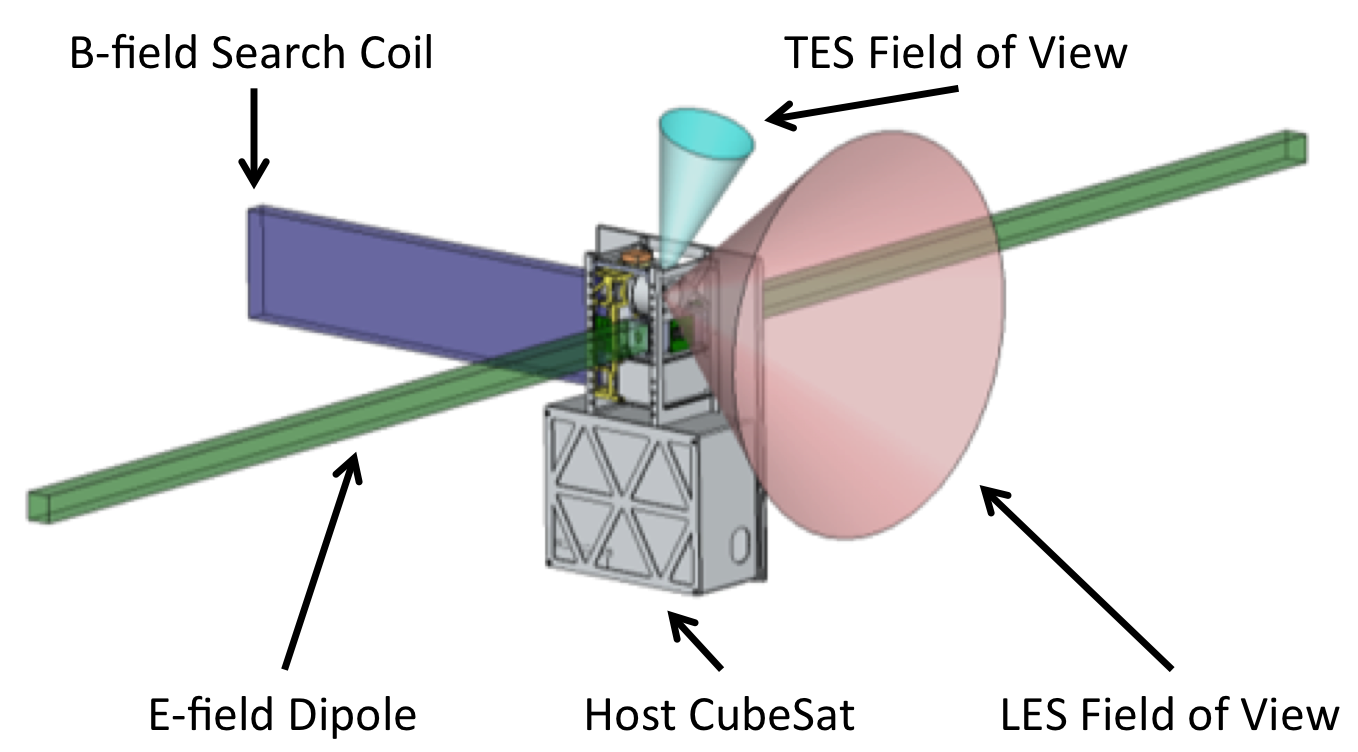
\includegraphics[width=20pc]{figures/vpm_figures/payload_figure_annotated.png}

\caption[Drawing of the assembled VPM payload on a 6U cubesat bus]{Drawing of an assembled VPM payload, shown in one possible configuration integrated into a 6U CubeSat bus, with both antennas deployed. Conical shapes indicate fields of view of the Lost-Electron Spectrometer (LES) and Trapped Electron Spectrometer (TES). }
\label{fig:VPM_full}
\end{center}
\end{figure}

\begin{figure}[t]
\begin{center}
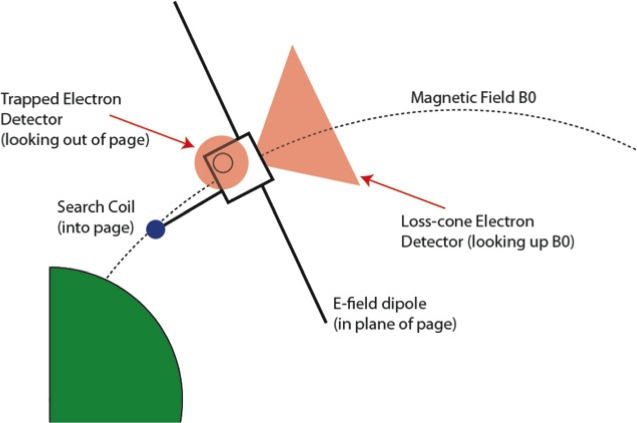
\includegraphics[width=20pc]{figures/vpm_figures/operations.png}

\caption[On-orbit alignment of the VPM payload]{Illustration of on-orbit alignment of the VPM payload. Conical, salmon-colored shapes indicate fields of view of the electron spectrometers; E and B fields are sampled perpendicular to each other and to the background magnetic field.}
\label{fig:operations}
\end{center}
\end{figure}




\section{Hardware Architecture}
VPM's system design was governed by three primary constraints:
\begin{enumerate}
\item Facilitate integration with a 3U CubeSat bus. The payload must fit into a 1.5U (10x10x15 cm) volume. The bus provides 3.3v and 5v power rails, an RS422 connection, and a single, 1-Hz-sampled analog connection.
\item Provide an upgrade path for high-reliability, radiation-tolerant components wherever possible.
\item Design simple operation modes with high reliability and low verification complexity. 
\end{enumerate}

The VPM payload consists of five hardware systems:
\begin{enumerate}
\item a power and interface board
\item a two-channel VLF broadband receiver ($\mu$BBR)
\item two deployable VLF antennas for sampling the electric and magnetic field respectively
\item a digital data processing system (DPU)
\item and a Loss-Cone Spectrometer (LCS), a pair of electron energy spectrometers designed to sample the energy distribution of the local loss cone. 
\end{enumerate}
All circuit boards are connected by a common stack connector and housed in an aluminum enclosure to reduce parasitic RF interference. A rendering of the system is shown in figure \ref{fig:hardware_stack}.

\begin{figure*}[htbp]
\begin{center}
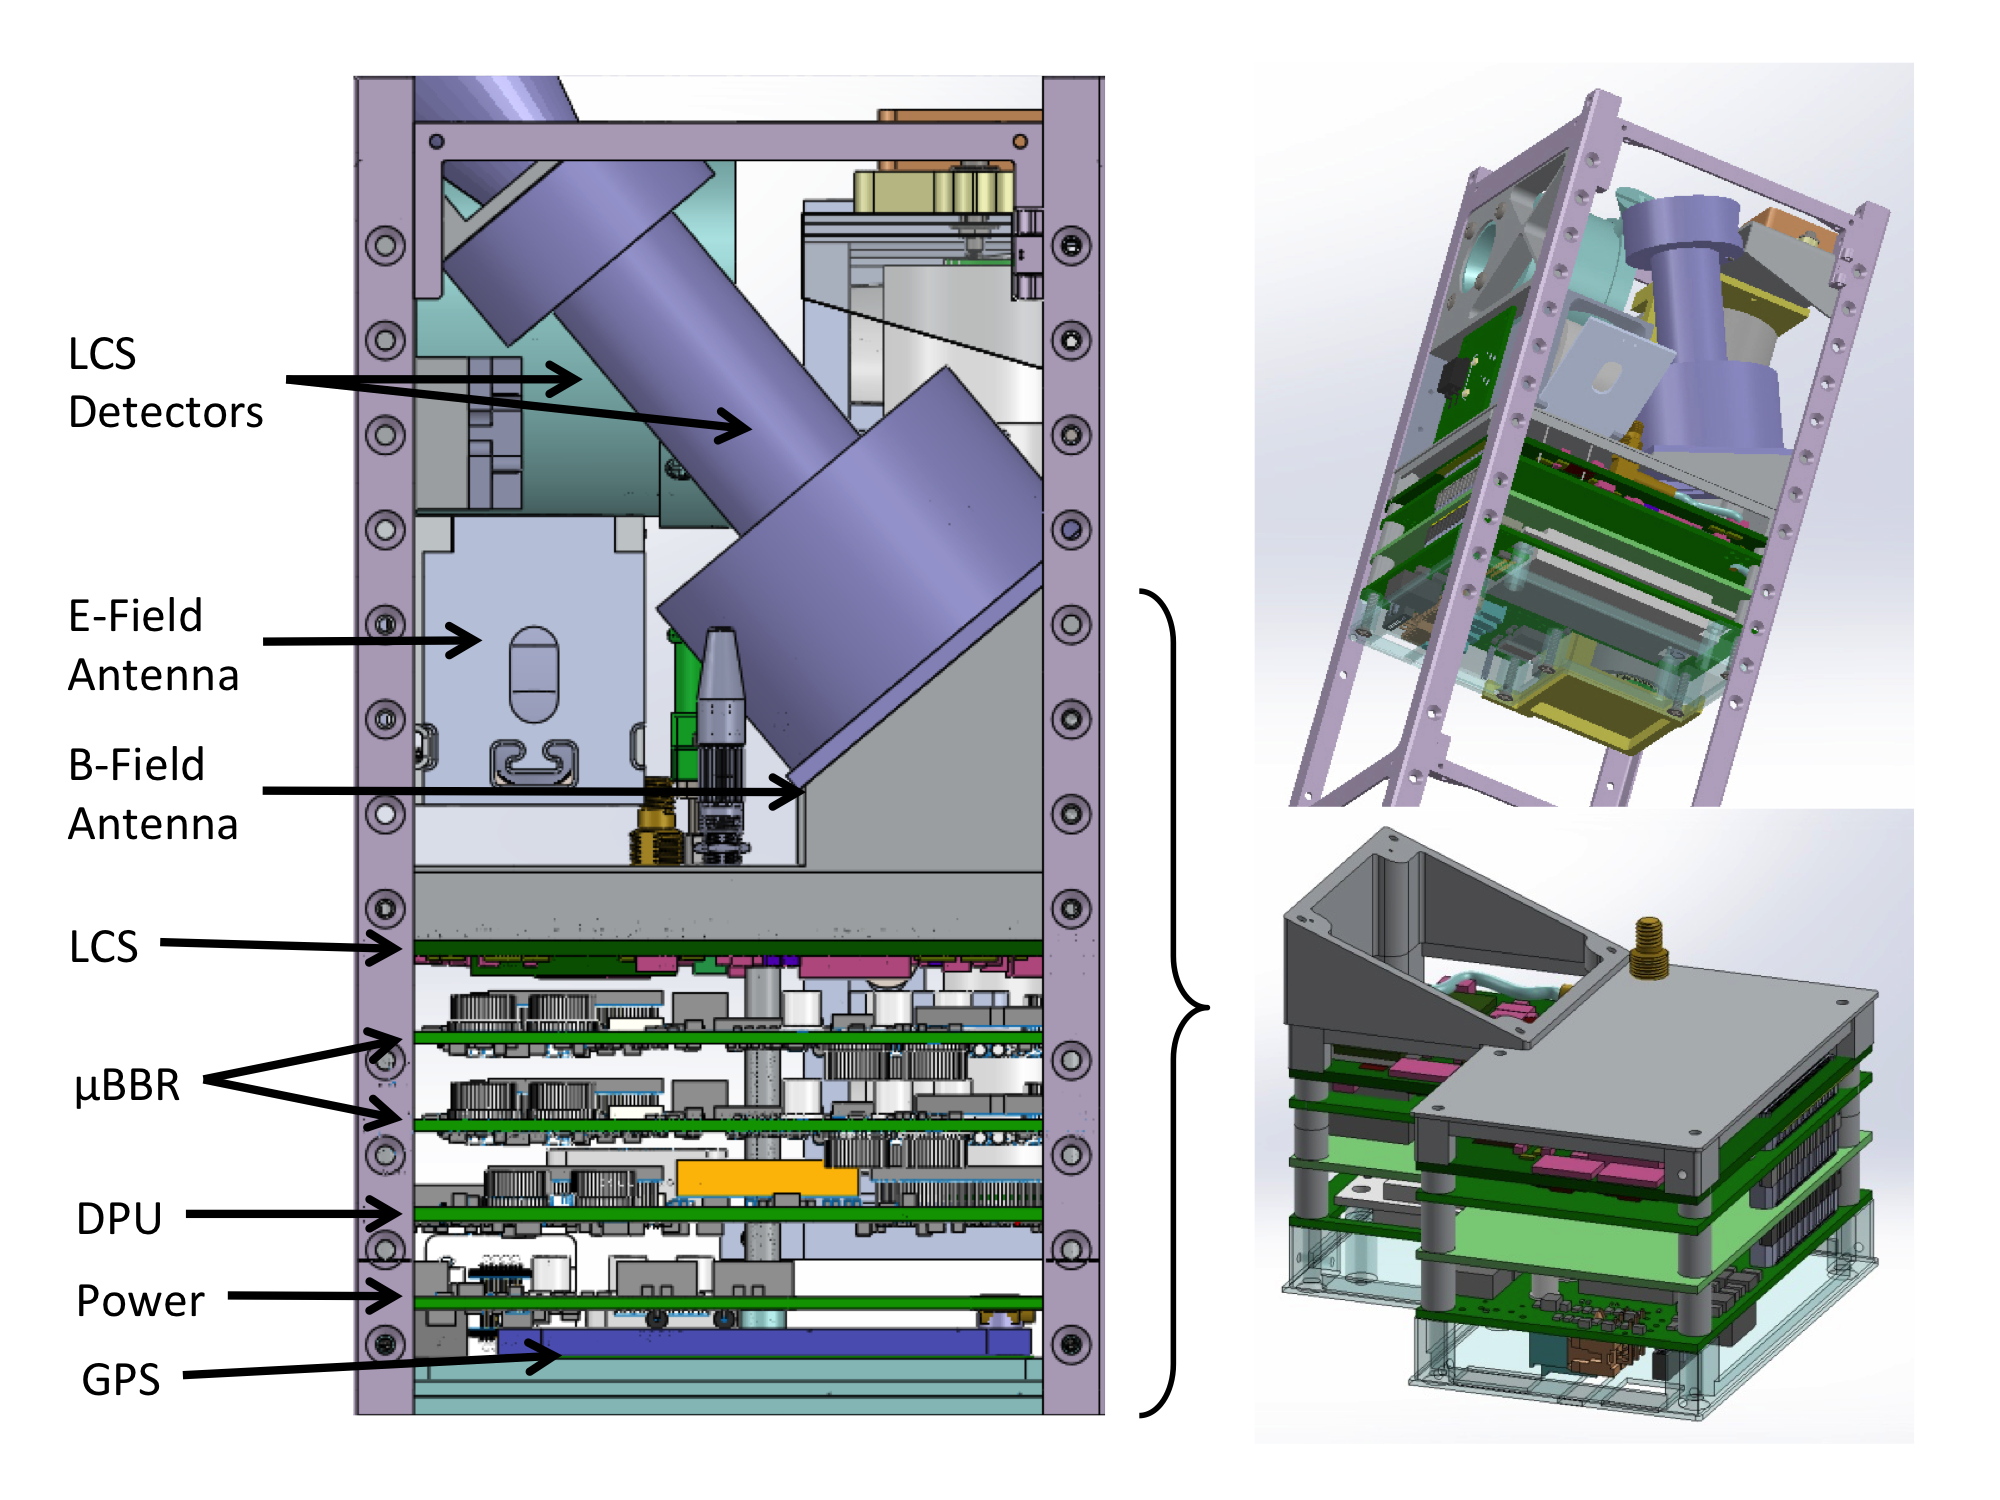
\includegraphics[width=32pc]{figures/vpm_figures/payload_figure.png}
\caption[VPM payload hardware instrument arrangement]{Rendering of the VPM payload hardware, showing locations of the E and B-field antenna deployers; the two particle detectors for the Loss-Cone Spectrometer, and the electronic card stack, shown without aluminum enclosure.}
\label{fig:hardware_stack}
\end{center}
\end{figure*}


\subsection{FPGAs}
Full-scale space systems commonly use radiation-tolerant, multiple-redundant single-board computers. While robust and flight-verified, such systems are cost, size, and power-prohibitive for a cubesat mission. Several commercial cubesat single-board computers exist (such as those from Pumpkin or Tyvak); however these systems are designed for general satellite operations, and provide more functionality than necessary for an isolated payload. Additionally, single-CPU solutions are not well-suited for realtime, parallel streaming tasks, as data from multiple sources must be buffered and processed serially, increasing memory and clock speed requirements. VPM omits any such embedded CPU and instead uses a realtime streaming solution implemented entirely in a Field-Programmable Gate Array (FPGA). 

FPGAs consist of a network of assignable logic gates and interconnections, which allow for gate-level circuits to be implemented using a hardware development language such as VHDL or Verilog, achieving ASIC-like performance without the burden of IC development. By working at the gate level, multiple-input designs can operate in clock-cycle-accurate lock step, allowing for low-power designs with minimal wasted circuitry. Additionally, gate-level designs inherently have fewer operating states, and once implemented, provide a high degree of reliability without risk of segmentation faults, memory leaks, or other higher-level issues common in CPU systems.

FPGAs find common use in embedded systems for peripheral interfacing and low-level data handling. A hybrid CPU / FPGA design was considered, wherein a ``soft" CPU is implemented within the FPGA fabric -- however such a design needlessly increased verification complexity, while similarly reducing system reliability. It should be noted, however, that VPM acts only as a peripheral for a separate satellite bus, and is not tasked with a myriad of other responsibilities required of a satellite mission -- telemetry, communication, power management and so forth -- the complexity of which necessitate a full CPU solution.

VPM uses the Actel ProAsic3 series of FPGAs. Actel FPGAs were selected largely for their focus on reliability, and simple upgrade path to a radiation-tolerant model. Development and prototyping was done using an A3PE/3000 chip (the largest available at time of design), which provides 3 million gates assignable in 75,264 tiles, and 604 kilobits of onboard SRAM . Additional functionality onboard the ProAsic3 series include clock conditioning circuits, differential signaling drivers, and 1 kilobit of flash ROM used to store lookup tables, which combined allow for a single-chip data processing system. %\citep{actel_a3pe_datasheet}.


\subsection{Power and GPS}
The lowest circuit board in the VPM stack houses power systems, antenna deployer drivers, and a GPS daughterboard. VPM requires three power connections from the host spacecraft -- +5v, +3.3v, and an unregulated, high-current-capacity supply at $\approx$ 9v, on a single micro-D connector. Additional connections are provided for two antenna deployers. A 100-pin stack connector is used for all inter-board power and communication.

VPM contains two deployable antennas -- a 1-meter flexible dipole antenna for sampling the electric field, and a magnetic-field search coil, which is deployed away from the system to reduce parasitic noise. Both antennas are tensioned and held in place using a burn-wire deployer in which a thin plastic filament is held against a conductive wire. To deploy, VPM drives a current through the wire until the plastic filament melts through, allowing the  antenna to extend on its own.

The power and GPS board contains two drive transistors to provide the necessary burn-wire current, and are fed from the unregulated supply. Connections are made to deployers via a pair of micro-D connectors.

Bipolar $\pm 12v$ power for the loss-cone spectrometer and searchcoil preamp is provided via a Picosat DC/DC converter. % \citep{picosat}. 

GPS timing and location are provided by a NovAtel OEM615 embedded GPS receiver. While not radiation-tolerant, this card has flight heritage on multiple CubeSat and nanosatellite missions, and can be configured to operate without altitude restrictions \citep{Spangelo2013}.

\subsection{DPU}
Data processing and system commanding is performed on the DPU board. The DPU board contains a single Actel A3PE/3000 FPGA housed in an FG484 ball-grid array package. Local power for the FPGA is supplied by linear regulator circuits -- 3.3v and 2.5v for IO banks, and switchable 1.5v or 1.2v for the FPGA core voltage, depending on whether an A3PE or A3PL part is populated. The FPGA is programmed through a 10-pin JTAG header.

Clocking onboard the DPU is provided by a 20 MHz temperature-controlled oscillator, which feeds a clock-conditioning circuit on the FPGA. Processing is done at a divided 10 MHz clock, with the exception of memory operations which operate at full speed.

Temporary data storage is provided by a 3D-Plus 128-megabyte SDRAM, which is clocked and controlled by firmware within the FPGA. The 3D-Plus SDRAM was selected primarily for availability of a pin-compatible, radiation-tolerant upgrade. The SDRAM uses a 32-bit wide data buss, and includes an internal refreshing algorithm.

Communication between VPM and the host satellite is implemented using a standard UART protocol over an RS422 connection, made through a pair of differential line drivers, again selected for a pin-compatible radiation-tolerant upgrade. % \citep{intersil_linedrivers}

VPM provides low-level housekeeping and debug signals over an analog connection, intended to be sampled by the host spacecraft. A variety of signals are connected through an analog multiplexing chip, including analog and digital power rails; system temperature as measured by a thermocouple near the GPS receiver; the bipolar 12v supply; and five channels allocated to the loss-cone spectrometer. Outputs can be selected via a system command, or set to cycle through at 5 seconds per input.

RS422 and analog housekeeping connections are made through a single micro-D connector. Connections are provided for an FTDI UM232H USB interface used extensively in development; however on flight, all connections are made through micro-D connectors or the 100-pin stack connector.

\subsection{VLF Receiver Boards}
VPM uses a modified version of the Stanford Micro Broadband Receiver ($\mu$BBR) as used on the SpriteSat mission, and the GLIMS payload onboard the International Space Station \citep{Ushio2011}. The VPM $\mu$BBR provides two channels of amplification, filtering, and digitization at an 80 kHz sampling rate. VPM uses a pair of proprietary chips -- a combination low-noise amplifier (LNA) and anti-ailiasing filter (AAF), and an analog-to-digital converter (ADC) -- which were the result of two PhD theses \citep{Wang2009, Mossawir2009}. The chips were designed for low power consumption and high radiation tolerance.

An intermediate buffering stage provides an additional 10 V/V gain; an active two-pole high-pass filter with a 3-dB point at 3 kHz can be inserted between the LNA and ADC sections, or bypassed completely using sealed, mechanical relays. Gain at the LNA can be remotely selected, either 1 or 10, for a total system gain of 20 or 40 dB. The assembled system gives a spurious-free dynamic range (SFDR) of approximately 55 dB across the passband. The analog stage operates on a single, 2.5v supply, which is derived locally using a 2.5v reference source and a radiation-tolerant op-amp. A simplified schematic of the receiver chain is shown in figure \ref{fig:ubbr_schem}.

\begin{figure*}[t]
\begin{center}
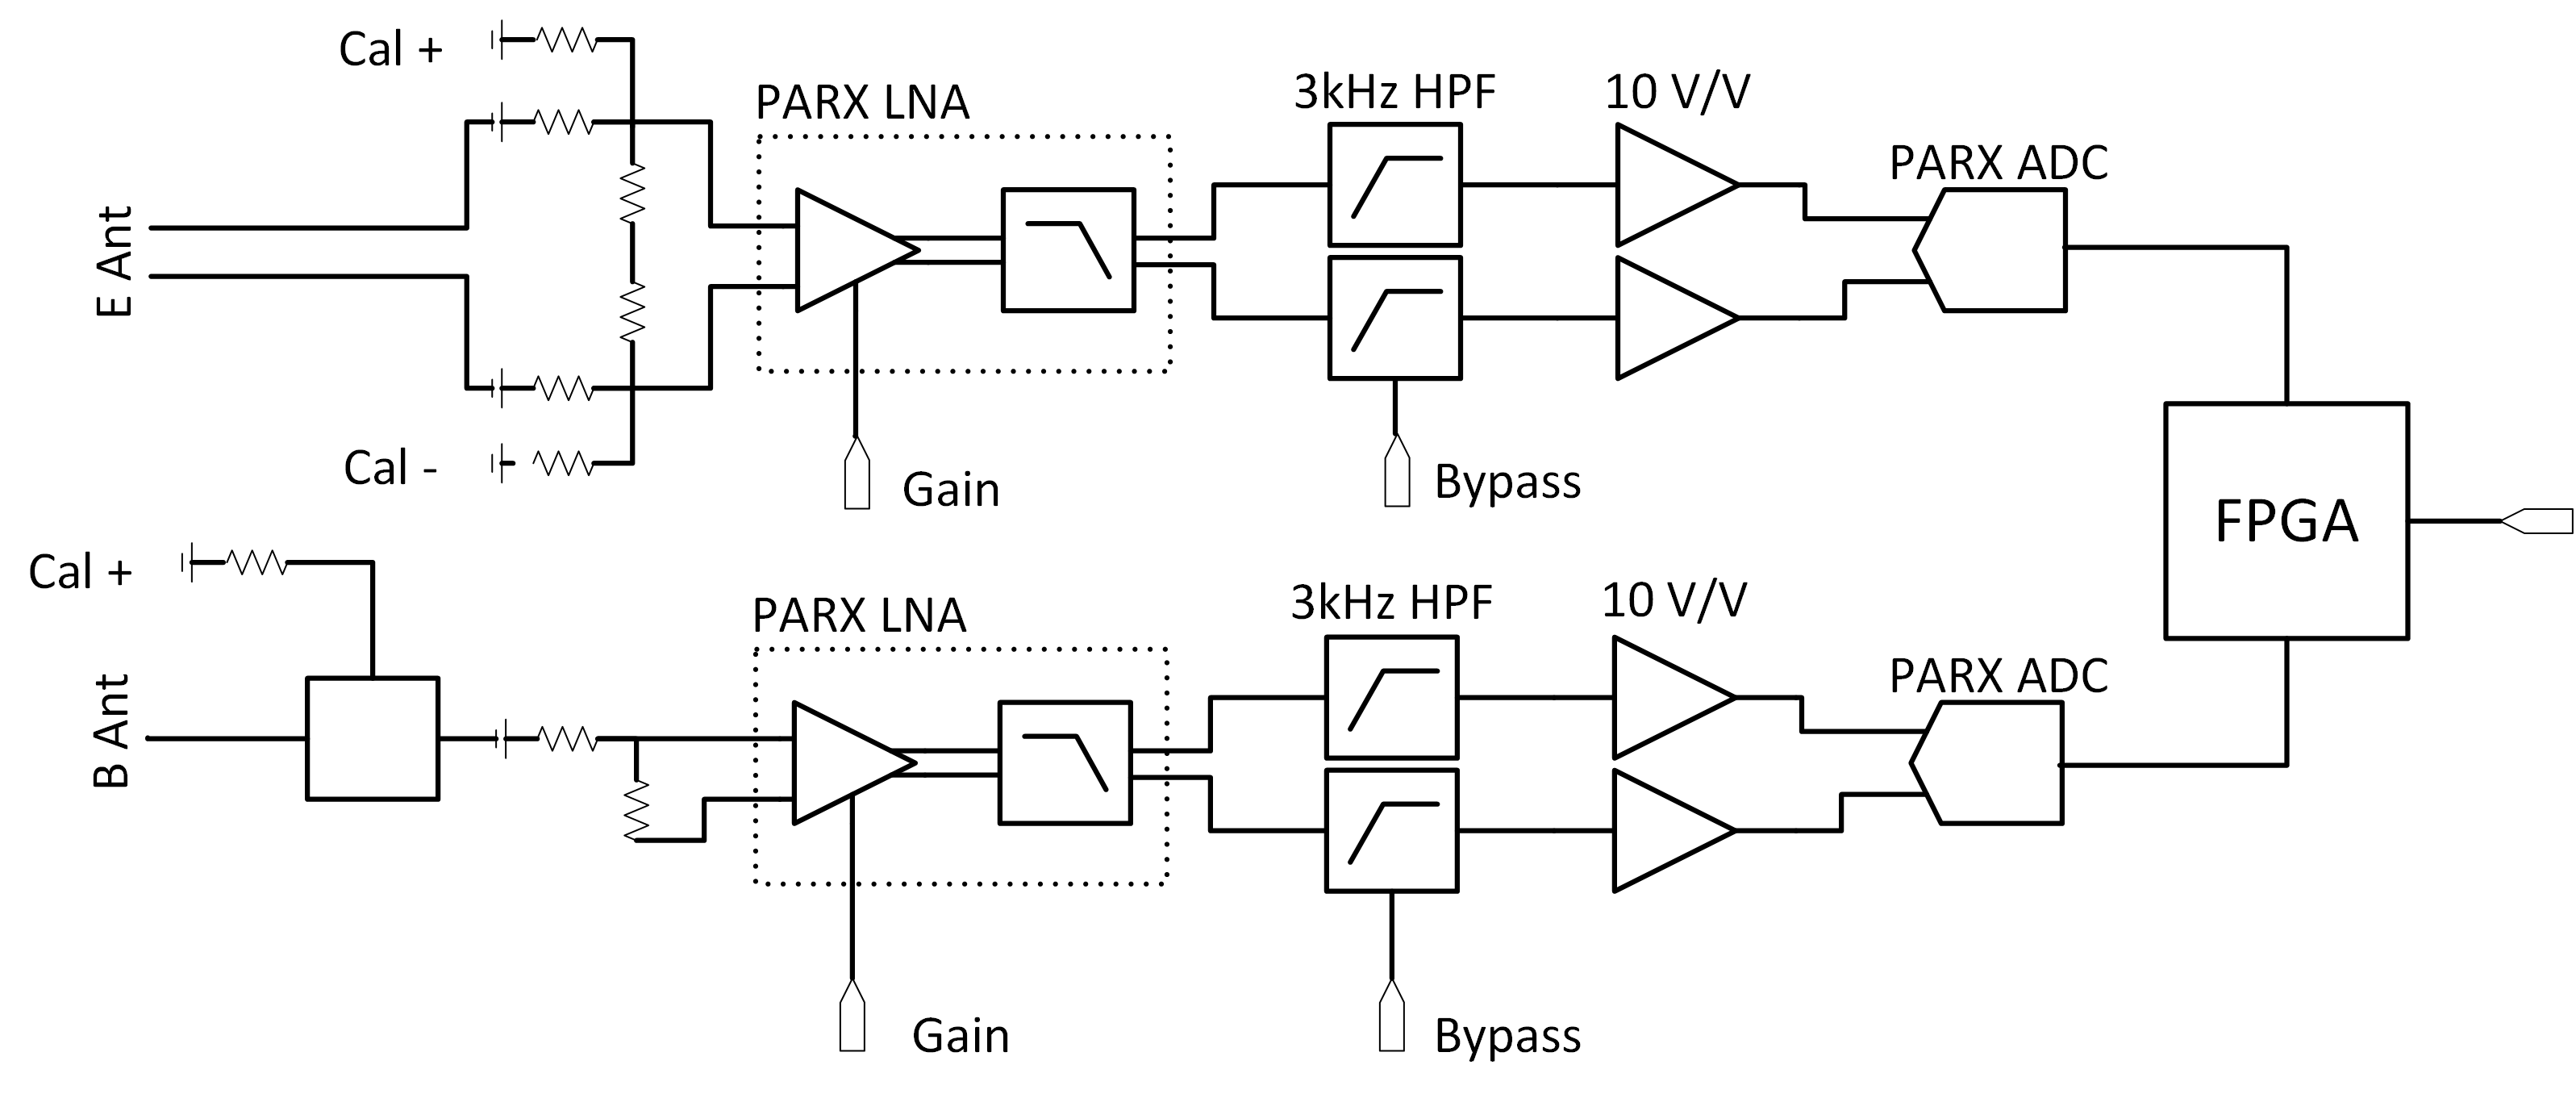
\includegraphics[width=35pc]{figures/vpm_figures/ubbr_schem.png}

\caption{Simplified schematic of the $\mu$BBR signal conditioning and data conversion chain}
\label{fig:ubbr_schem}
\end{center}
\end{figure*}

Channel 1 features a differential input, which is capacitively coupled to the electric dipole antenna. Channel 2 is single-ended, and connects to the output of a magnetic-field search coil, which contains its own active signal conditioning circuitry. Filtering and amplification is done differentially, using parallel single-ended circuits. 

The ADCs use a 5-stage pipeline architecture; digital assembly and calibration of the first three stages is performed in an FPGA. The resulting FPGA module returns 13-bit equivalent resolution, packed as 16-bit samples \citep{Wang2009}. 

Signal conditioning and ADC are located on a single board, which feed an interstitial FPGA on a second board. Parasitic coupling between the two channels is reduced by constraining each channel to a separate side of the board, with a ground-plane layer separating the two. 

The $\mu$BBR FPGA receives system and sampling clocks through the 100-pin stack connector, by way of the DPU FPGA. When enabled, the 80 kHz sampling clock is generated by the GPS card and is accurate to $\pm$50 nanoseconds. Should the system fail to detect a GPS-synchronized clock for more than 6 seconds, the system will attempt to reset the GPS card. If three resets are attempted without success, the system will default to an internally-generated sampling clock, which is derived from an onboard oscillator. GPS synchronization can be re-enabled via a system command.

All digital communication between the $\mu$BBR and the DPU is done via differential (LVDS) signaling. All communication is done synchronous to the DPU system clock, to eliminate communication errors due to clock and temperature drift.


 \subsubsection{Calibration Tone}
The $\mu$BBR signal chain features an onboard calibration signal generator, which can be used to assess the frequency response of the system on-orbit. A pseudorandom digital signal is generated using the $\mu$BBR FPGA, using the feedback register methodology described by \cite{Paschal2005}. VPM uses a 7-bit feedback register for a maximal-length sequence of 128 samples. This signal is passed through a voltage divider and capacitively coupled to the input of each analog channel. The Fourier transform of the resulting signal features a comb of uniformly-spaced frequencies, as shown in figure \ref{fig:caltone}. When calibration mode is entered, the system will generate one minute of calibration tone, which can be recorded by a 30-second, full-resolution burst. Results of a typical calibration are shown in figure  \ref{fig:bbr_calibration}.

Finally, an onboard digital sine-wave generator can be enabled; in this mode the $\mu$BBR ignores any analog signal and delivers a full-scale sine wave. While not scientifically useful, this mode enables diagnosis of communications issues, and confirmation of survey-mode processing.

\begin{figure}[ht]
\begin{center}
\includegraphics[width=20pc]{figures/vpm_figures/caltone.eps}

\caption[Pseudo-random calibration signals]{Pseudorandom calibration signal. Plot (a) shows two repetitions of the signal in the time domain, with magnitude attenuated from the 3.3v LVDS pin; plot (b) shows the Fourier transform of the signal. Red circles denote total power summed from adjacent frequency bins, to account for windowing effects.}
\label{fig:caltone}
\end{center}
\end{figure}

\begin{figure}[t]
\begin{center}
%\includegraphics{Figures/gain_logfreq.eps}
%\includegraphics{Figures/noisefloor_logfreq.eps}
\includegraphics[width=20pc]{figures/vpm_figures/gain_noise_combined.eps}
\caption[Frequency response and noise floor of the $\mu$BBR analog processing chain]{Characteristics of the $\mu$BBR analog signal conditioning chain, beginning with the LNA/AAF.  Plot (a) shows the frequency response for both high and low gain settings. Responses of the antennas are not taken into account. Selectable high-pass filters are disabled. Plot (b) shows the power spectrum of the noise floor, which is effectively independent of gain setting. Level is in decibels relative to $\pm$ 1.0 volts full-scale.}
\label{fig:bbr_calibration}
\end{center}
\end{figure}



\subsection{Deployable Antennas}
VPM contains two deployable antenna structures, oriented perpendicular to each other and to the background magnetic field, which facilitate discrimination of electromagnetic waves from evanescent fields. The electric dipole antenna was designed by the Deployable Structures team at the Air Force Research Lab (AFRL), while the magnetic field antenna and apparatus was designed by the French Climate Research Laboratory at the National Center for Scientific Research (CNRS).

The electric dipole antenna is comprised of a conductive strip on a flexible tape, which is rolled up and held in place with a burn wire. 

%Analysis of an electrically-short dipole antenna in free space is straightforward and efficient: For an incident plane wave, the antenna can be modeled as an equivalent voltage source with $V=\|E_0\| sin(\theta)l_{eff}$, where $E_0$ is the magnitude and time-varying component of the electric field; $\theta$ is the angle between the wave vector and the antenna; and $l_{eff}=L/2$ is the effective length of the dipole element. This source is in series with an equivalent resistance given by:
%\begin{equation}
%R_{ant} = \frac{2 \pi}{3} \eta_0 (\frac{l_{eff}}{\lambda})^2
%\end{equation}

%where $\eta_0 = 377 \Omega$ is the characteristic impedance of free space, and $\lambda$ is the wavelength \cite{elliot_antennas}.

%Within the VLF band, the dipole resistance becomes trivially small. The antenna is capacitively-coupled to the $\mu$BBR input terminals, with a DC rolloff at 1 Hz. Assuming an infinite plane wave with right-angle incidence and ignoring plasma effects, the conversion between input voltage at the $\mu$BBR terminals and electric field magnitude $V_{in}/E_0$ (Volts per Volts / meter) is $\approx$ 1.

In the presence of a plasma, the electric dipole antenna's impedance can vary substantially with plasma parameters (density, temperature), and orientation with respect to the background magnetic field. For analytic, closed-form expressions, see \cite{Balmain1964}, and thethe series of papers by Wang and Bell \citep{Wang1969, Wang_Bell_1972}. For a full numerical treatment of plasma-immersed VLF electric dipoles, see the thesis work of Chevalier \citep{Chevalier2007}. 

For purposes of system characterization, we assume the antenna and receiver are perfectly matched; assuming an infinite plane wave with right-angle incidence and ignoring plasma effects, the conversion between input voltage at the $\mu$BBR terminals and electric field magnitude $V_{in}/E_0$ (Volts per Volts / meter) is $\approx$ 1.

The search-coil antenna is also deployed from the payload to reduce electrical interference. The antenna includes a dedicated preamp which operates on $\pm$12v power. Sensitivity of the antenna and preamplifier are shown in figure \ref{fig:searchcoil}.

Both antennas use a single-deploy burn-wire system. VPM includes options for each deployer to be armed and deployed separately, and can be repeated in the event that the retaining filament fails to release the antenna.

Deployed antennas are shown in figure \ref{fig:VPM_full}.

Figure \ref{fig:detectable_ranges} gives a rough estimate of the maximum and minimum detectable field amplitudes. Maximum levels are calculated assuming the low gain setting and a clipping voltage at the ADC; minimum levels are those which are below the system's noise floor at the high gain setting. Note that, for a plane wave in free space, the magnitudes of E and B are related by $B_0 = \frac{E_0}{c}$, where c is the speed of light; For an electric field $E_0 \approx 1$ V/m, the corresponding magnetic field has $B_0 \approx 0.3$ nT.

The range of measurable amplitudes is comparable to other in-situ VLF measurement systems; DEMETER reports a minimum sensitivity of $2\times10^{-5}$nT-Hz$^{-1/2}$ \citep{Cussac2006}. The Electric Fields and Waves (EFW) instrument onboard the Radiation Belt Storm Probes (RBSP) satellite use 100-meter double probe sensors with a maximum detection amplitude of $\pm 1$ V/m \citep{Wygant2014}. Several other studies report phenomena within the VLF band (whistlers, chorus) to have amplitudes on the order of 20 mV/m and 1 nT \citep{Wygant2014, Cattell2015, Bhattacharya2009}.



\begin{figure}[t]
\begin{center}
\includegraphics[width=20pc]{figures/vpm_figures/searchcoil_response_2up.eps}
\caption[Characteristics of the search coil and associated preamp]{Characteristics of the search coil and associated preamp. Plot (a) shows the transfer function in dB-scaled volts per nanotesla. Plot (b) shows the search coil and preamp's noise spectral density in units of nanotesla per $Hz^{1/2}$}
\label{fig:searchcoil}
\end{center}
\end{figure}


\begin{figure}[t]
\begin{center}
%\includegraphics{Figures/detectable_ranges.eps}
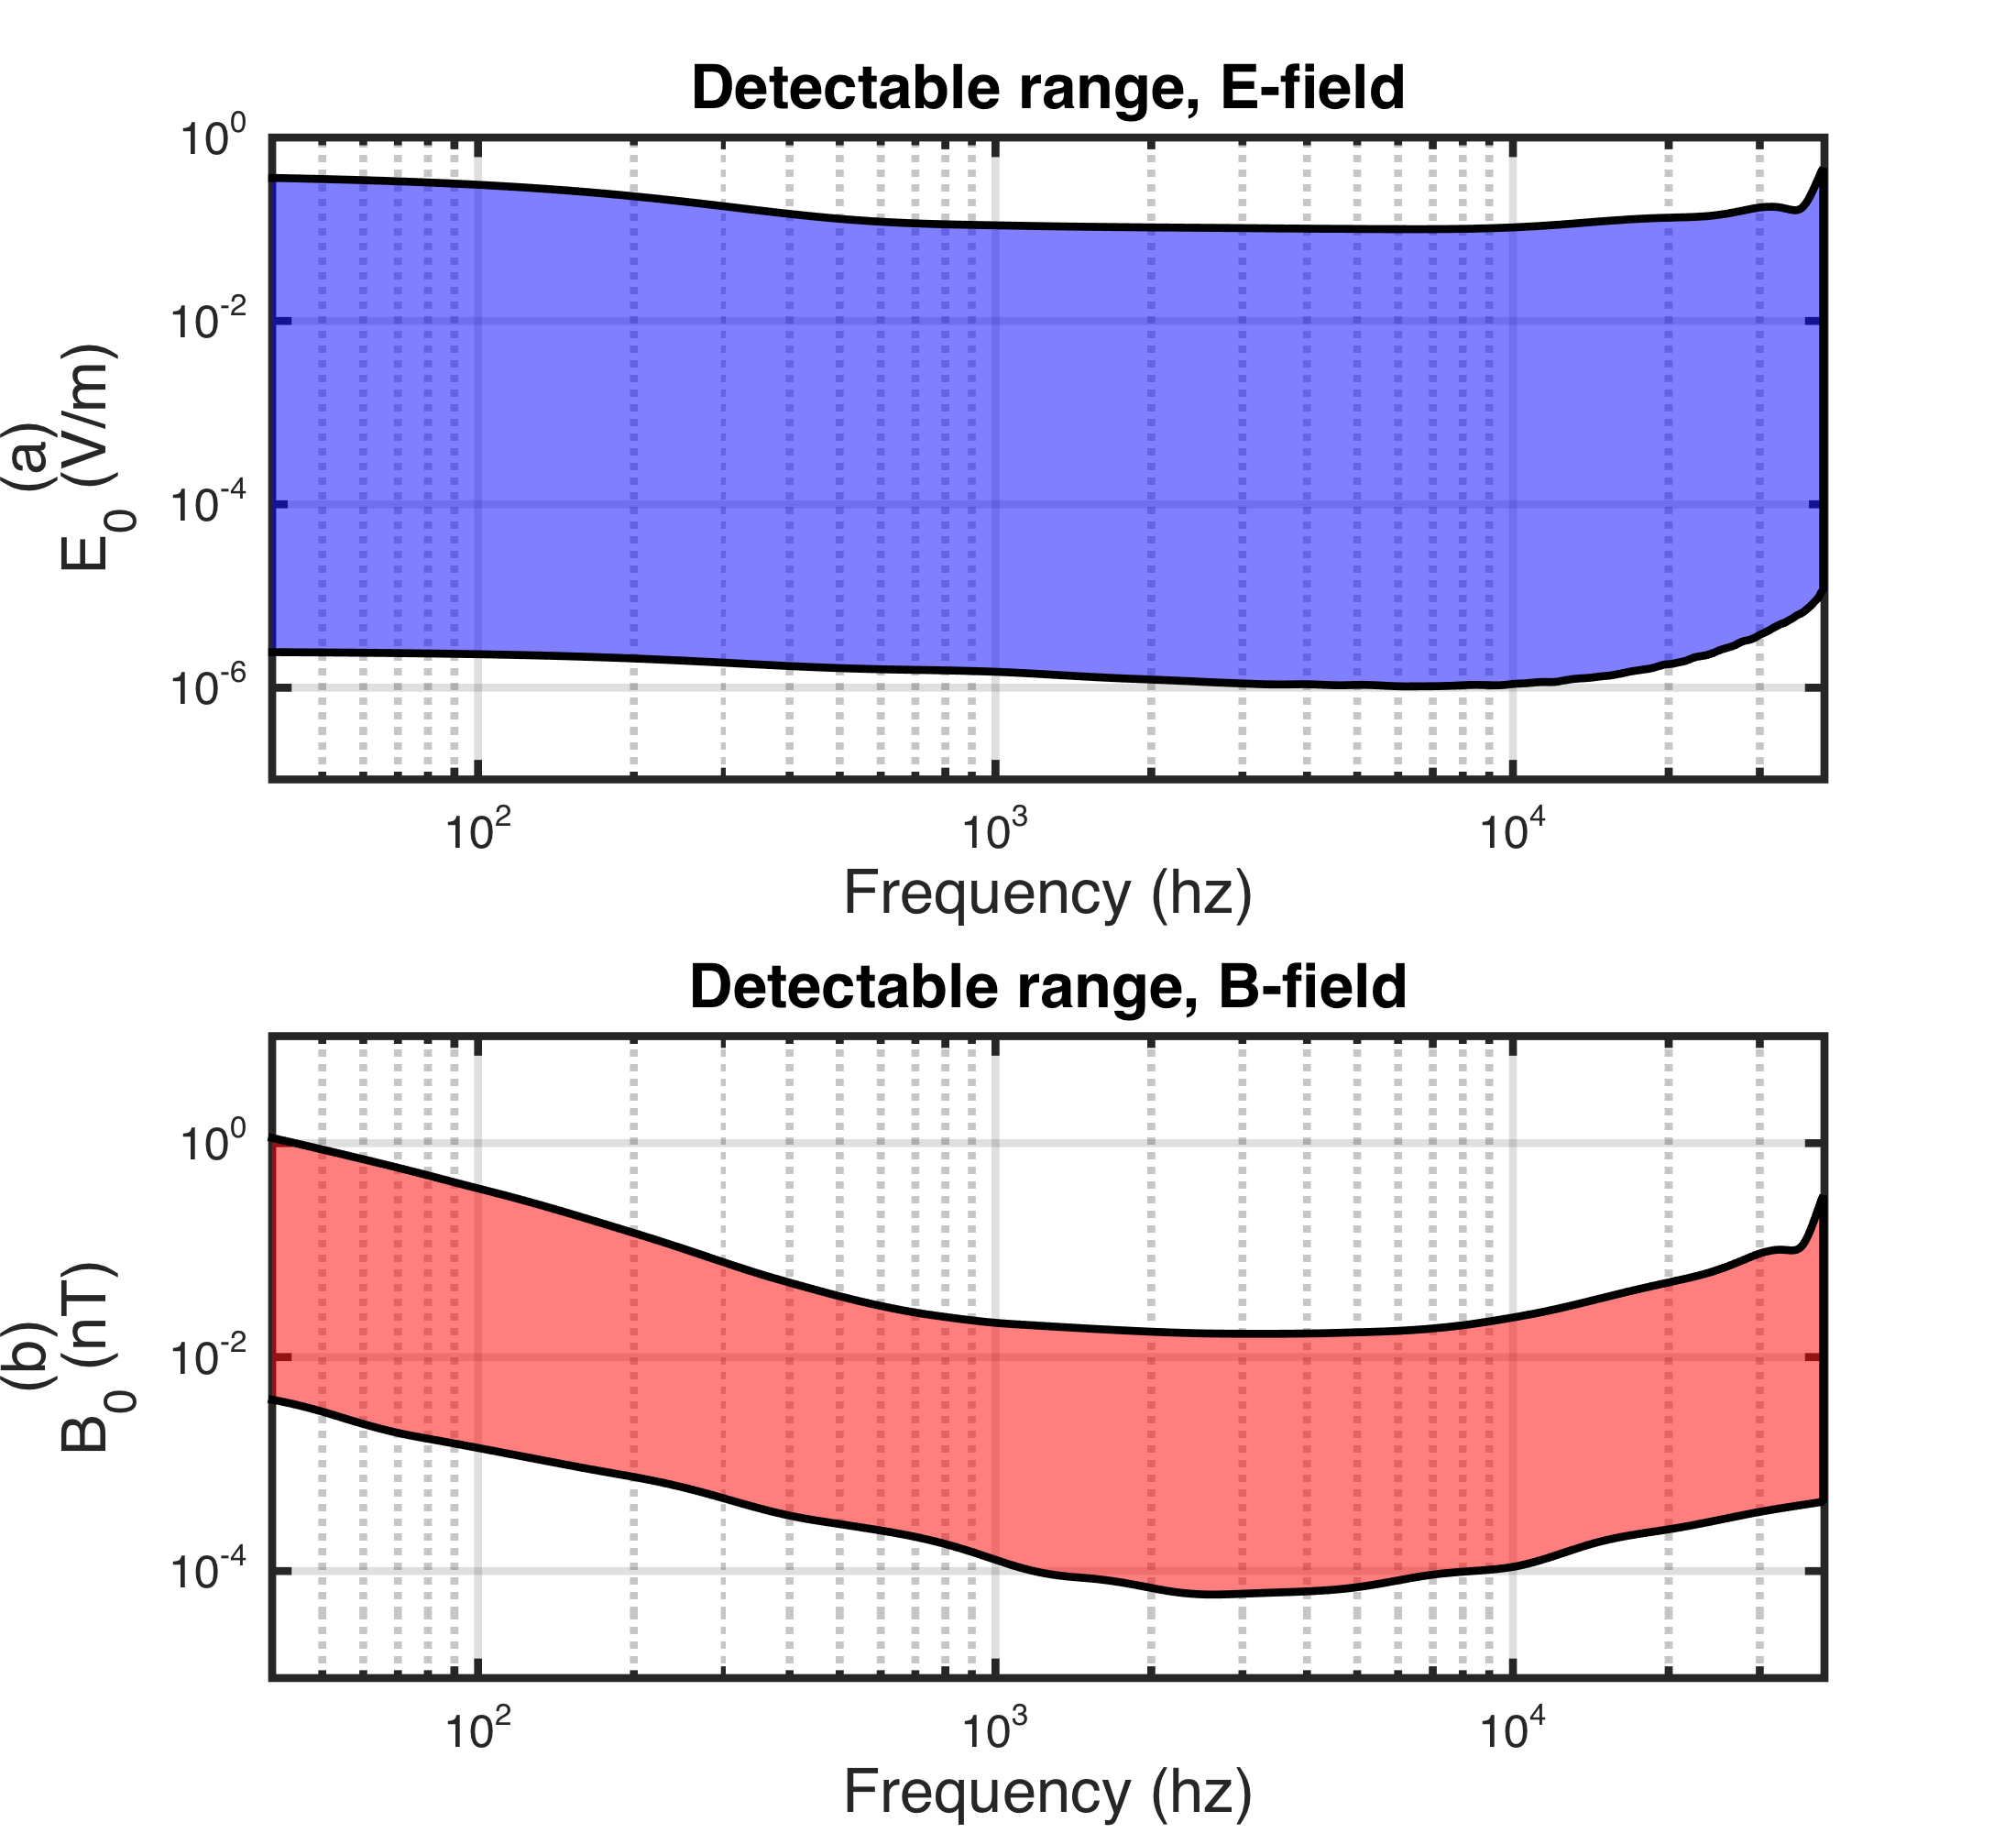
\includegraphics[width=20pc]{figures/vpm_figures/detectable_ranges.png}

\caption[Approximate detectable field magnitudes]{Approximate detectable field magnitudes, assuming no loss due to geometric factors of the antennas. Plot (a) shows the range of electric field strengths $E_0$ in Volts / Meter. Plot (b) shows the range of magnetic fields in nanotesla.}
\label{fig:detectable_ranges}
\end{center}
\end{figure}


\section{Firmware Architecture}
\begin{figure*}[t]
\begin{center}
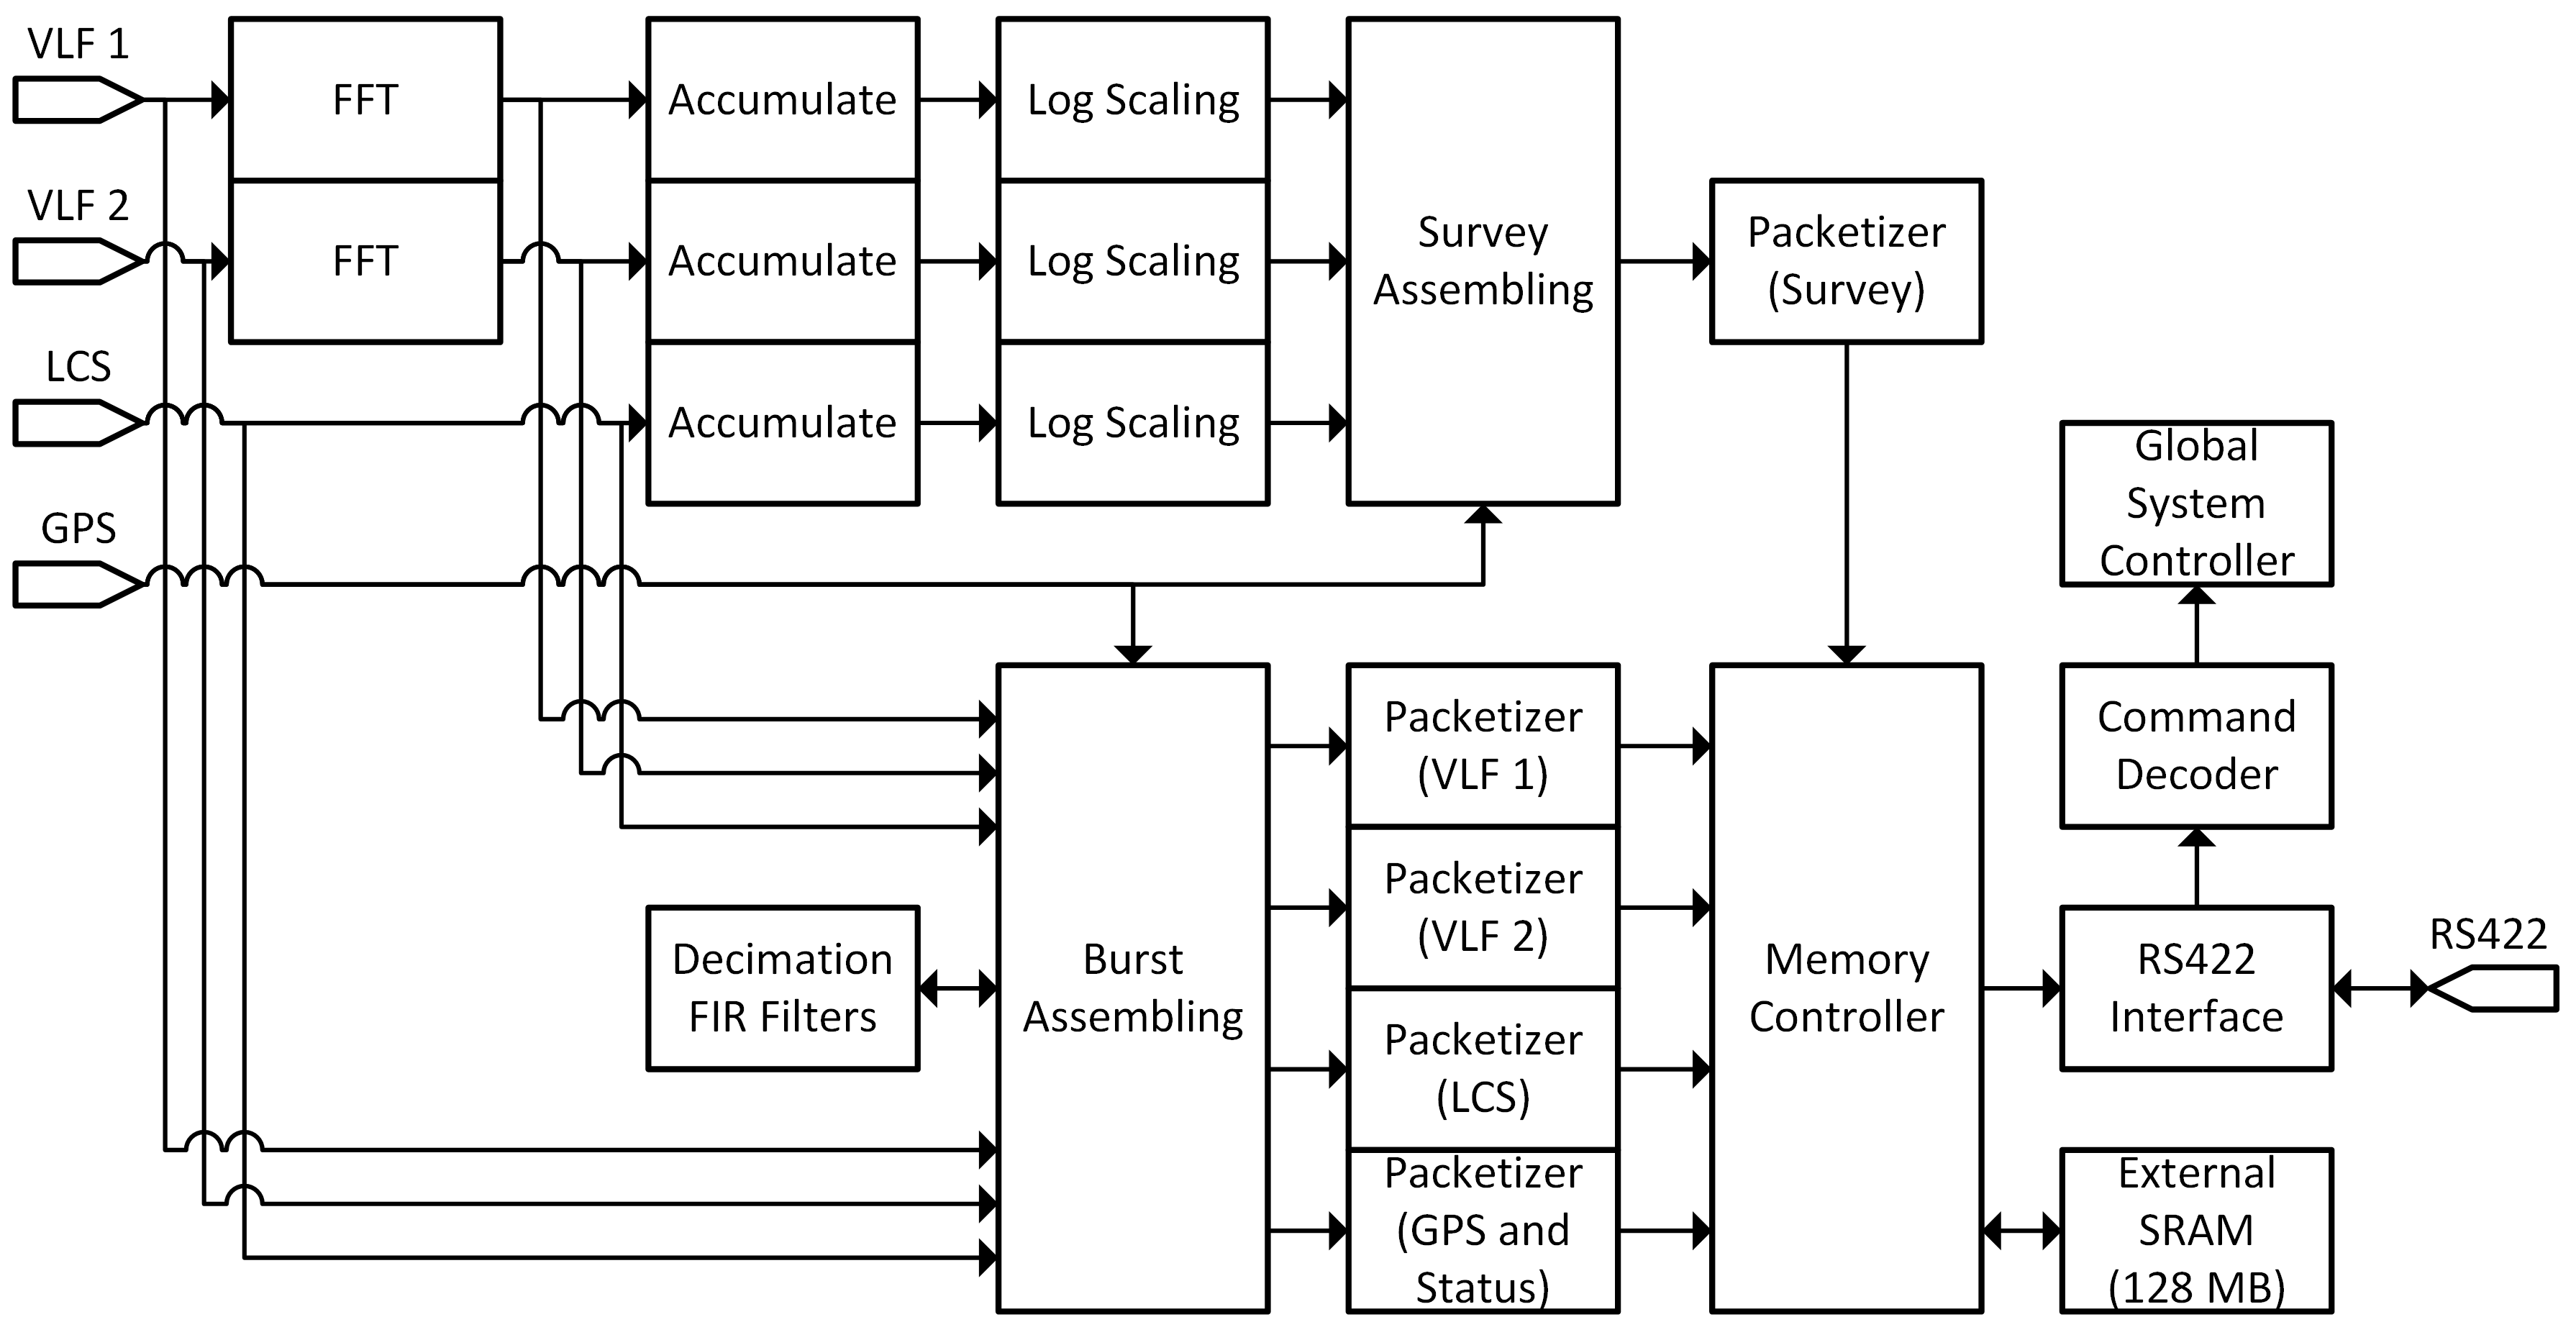
\includegraphics[width=35pc]{figures/vpm_figures/firmware_diagram_v2.png}

\caption[Block diagram of VPM firmware modules]{Block diagram of firmware modules. Arrows indicate flow of data.}
\label{fig:firmware_arch}
\end{center}
\end{figure*}
VPM delivers two data products -- a low-resolution survey mode, which runs constantly, and a commandable burst mode, which will accumulate an equivalent of 30 seconds of full-resolution data. All data processing is performed on a single Actel ProAsic3 FPGA, using fixed-point, twos-compliment arithmetic. Survey and burst mode streams operate in parallel, feeding data to a common memory controller, which packetizes and buffers data using a radiation-tolerant 128MB SDRAM. Fixed-size packets are then transmitted at the soonest availability to the host spacecraft at 400 kilobaud using a standard RS422 / UART protocol.

Figure \ref{fig:firmware_arch} shows a block diagram of the firmware architecture.


\subsection{Reduced-Resolution (Survey) Data}
Survey data consists of a reduced-resolution energy spectrogram for each VLF channel, and if installed, an energy histogram of each particle detector. Survey-mode time resolution can be selected from one of three presets -- short, medium, and long -- corresponding to 1024, 2048, or 4096 FFTs, or 6.5536, 13.1072, or 26.2144 seconds respectively. VLF spectrograms consist of 512 frequency bins, with energies mapped to 8 bits on a logarithmic scale.

\subsubsection{Frequency Mapping and Accumulation}
VLF data is delivered to the DPU as 16-bit, twos-compliment integers, which are buffered locally, overlapped by 50\% (512 samples), and multiplied by a Chebyshev window function. Data is then mapped to the frequency domain using a 1024-point, decimation-in-time Fast Fourier Transform, as described in \citep{Oppenheim_Schafer}. Buffering within the FFT is sized such that the full resolution of multiplications are kept without overflow. Real and imaginary components are rounded to 16 bits.

Absolute values of the real and imaginary components are then squared and summed, resulting in a 512-point vector of 32-bit integers, representing the squared magnitude of the frequency content.

Magnitudes are then accumulated using the full input resolution plus 12 padding bits, guaranteeing no overflow for $2^{12} = 4096 $ accumulations. The resultant output is a 512-point vector of 44-bit integers.

\subsubsection{Fixed-Point Log Scaling}
Arithmetic beyond addition, subtraction, multiplication, and power-of-two division is intractable without a dedicated arithmetic unit, generally requiring an iterative or multi-cycle algorithm. In many cases a simple lookup table can be used to map values from one space to another; however the size of a stored lookup table can become unwieldy with increased resolution. VPM makes use of a hybrid algebraic / lookup table method to map 44-bit integers to an 8-bit logarithmic space in a single clock cycle, and making efficient use of FPGA resources.

We begin with the log-of-sums identity:
\begin{equation}
\rm{log}_{n}(a + b) = \rm{log}_n (a) + \rm{log}_n(1 + \frac{b}{a})
\end{equation}
where we separate our input into the \emph{integer} portion, $a$, and the \emph{fractional} portion, $b$. We take the integer portion to be the maximum power of two less than the input, and the fractional portion to be the remainder, $b = x - a$. Each component can then be dealt with separately via a reduced lookup table.

The integer portion is simple to compute: $\rm{log}_2({2^{n}}) = n$, which can be calculated by finding the index of the greatest nonzero bit. To make full use of 8 output bits, we multiply by a scaling factor given by:
\begin{equation}
S = \frac{2^{Nb_{out}}}{Nb_{in}}
\end{equation}

Where $Nb_{out} = 8$, the number of bits at the output, and $W_{in} = 32$, the number of bits at the input, for a scaling factor of $S = 8$.

The fractional portion, $\rm{log}_2(1 + \frac{b}{a})$ is determined using a lookup table with $2^{Nb_{frac}}$ entries.

This method makes most-efficient use of the output range when both input and output bit widths are powers of two -- e.g., mapping 32-bit input to 8-bit output. Using $Nb_{in} = 32$, $Nb_{out} = 8$, and $Nb_{frac} = 5$, we require only two 32-entry lookup tables, rather than an intractable $2^{32}$ entries for a direct lookup table, or 256 entries for a partitioning lookup table.

VPM's accumulators deliver 44-bit integers, which must be passed into the 32-bit lookup tables. However, by simply taking the 32 most-significant bits, we introduce substantial error in the smaller output values. In order to make full use of the 44-bit integers, we use a barrel-shifting technique using the log-of-products identity:
\begin{eqnarray}
\rm{log}(ab) = \rm{log}(a) + \rm{log}(b) \\
\rm{log}(\frac{a}{b}) = \rm{log}(a) - \rm{log}(b) 
\end{eqnarray}

In the event that simply taking the most-significant 32 bits will result in a truncated fractional portion, we shift the input by $Nb_{frac}$ bits; equivalent to multiplying by $2^{Nb_{frac}}$. We then pass the top 32 bits to the lookup tables, sum the result, and subtract the added portion $S\cdot Nb_{frac}$. The complete module is shown in figure \ref{fig:logscaling}, and performs within $\pm 1$ bit from the equivalent floating-point computation in Matlab when $x$ is greater than $2^{12} = 4096$.



For each frequency, the equivalent survey-mode computation is given by:
\begin{equation}
{\rm round}(S \cdot {\rm log}_2(\frac{1}{n}\sum_1^n{(\rm{re}(x_f)^2 + \rm{im}(x_f)^2)})
\end{equation}
where $x_f$ are the outputs of the windowed, overlapped FFT.


\begin{figure}[htbp]
\begin{center}
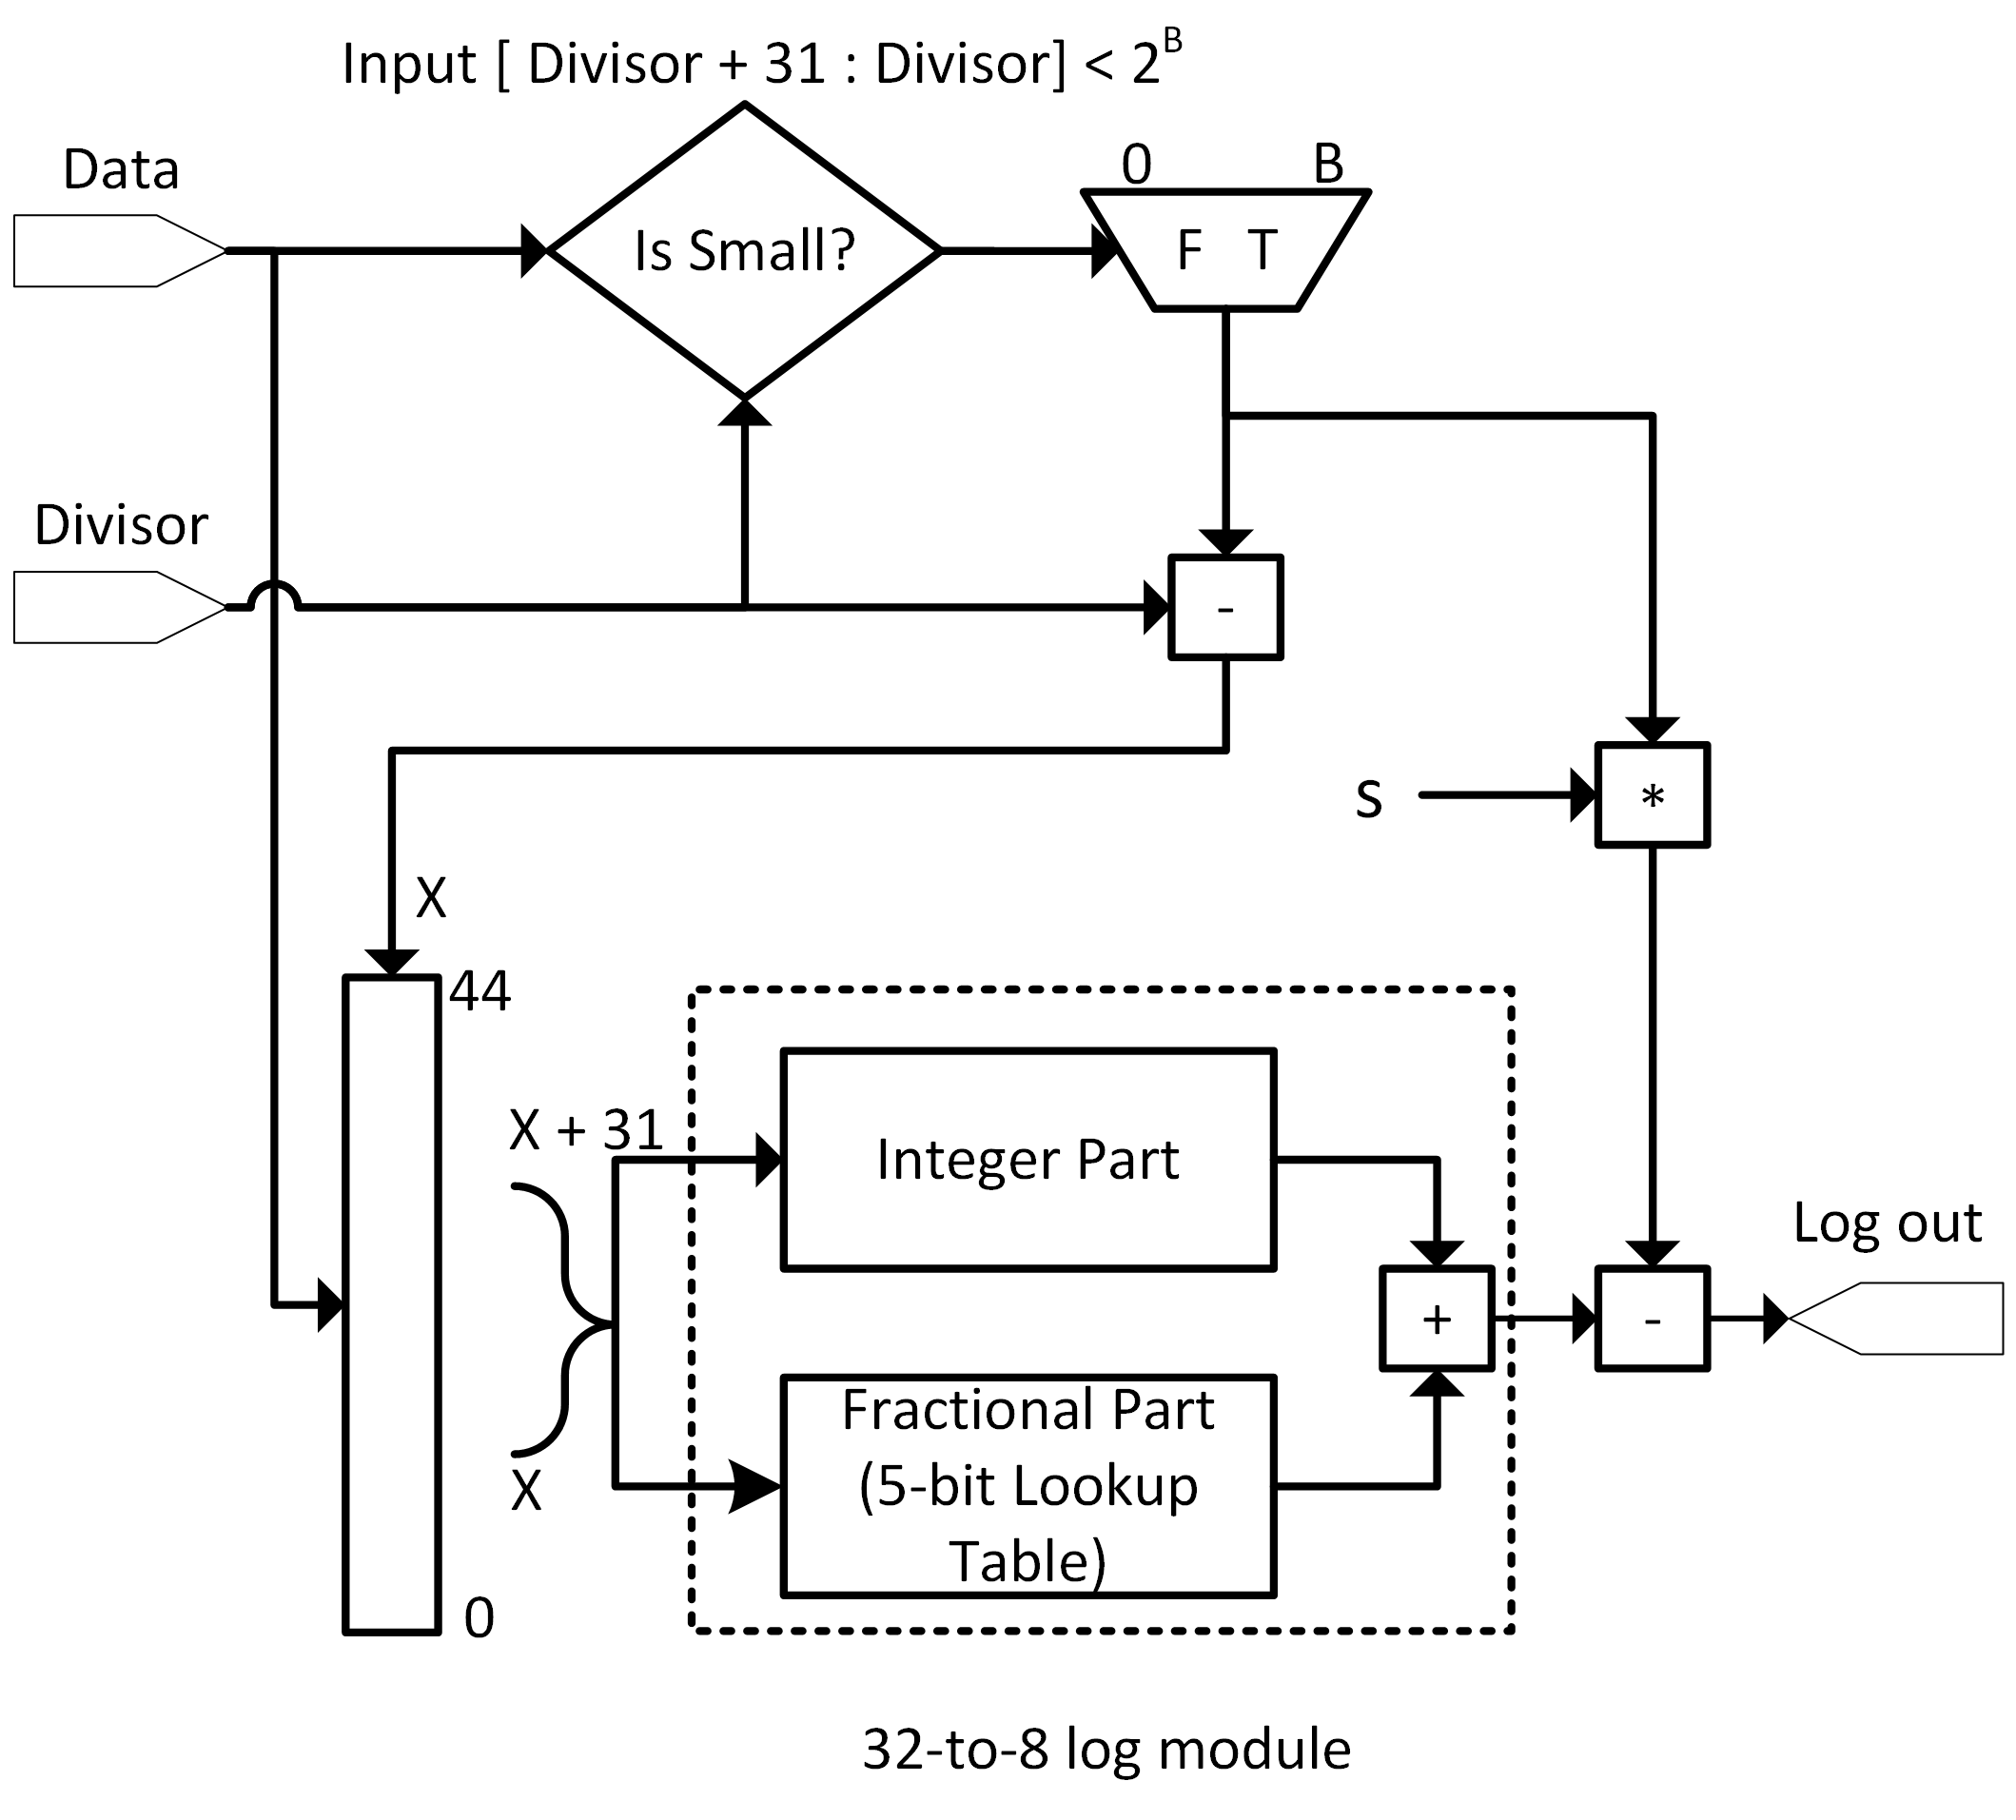
\includegraphics[width=20pc]{figures/vpm_figures/log2_v5.png}

\caption[Block diagram of the fixed-point log scaling module]{Block diagram of the log-scaling module, which efficiently maps a 32-bit average to an 8-bit value. Additional logic improves accuracy by making use of truncated bits for small inputs.}
\label{fig:logscaling}
\end{center}
\end{figure}

\subsubsection{Survey Product Data Structure}
\begin{figure}[h]
\begin{center}
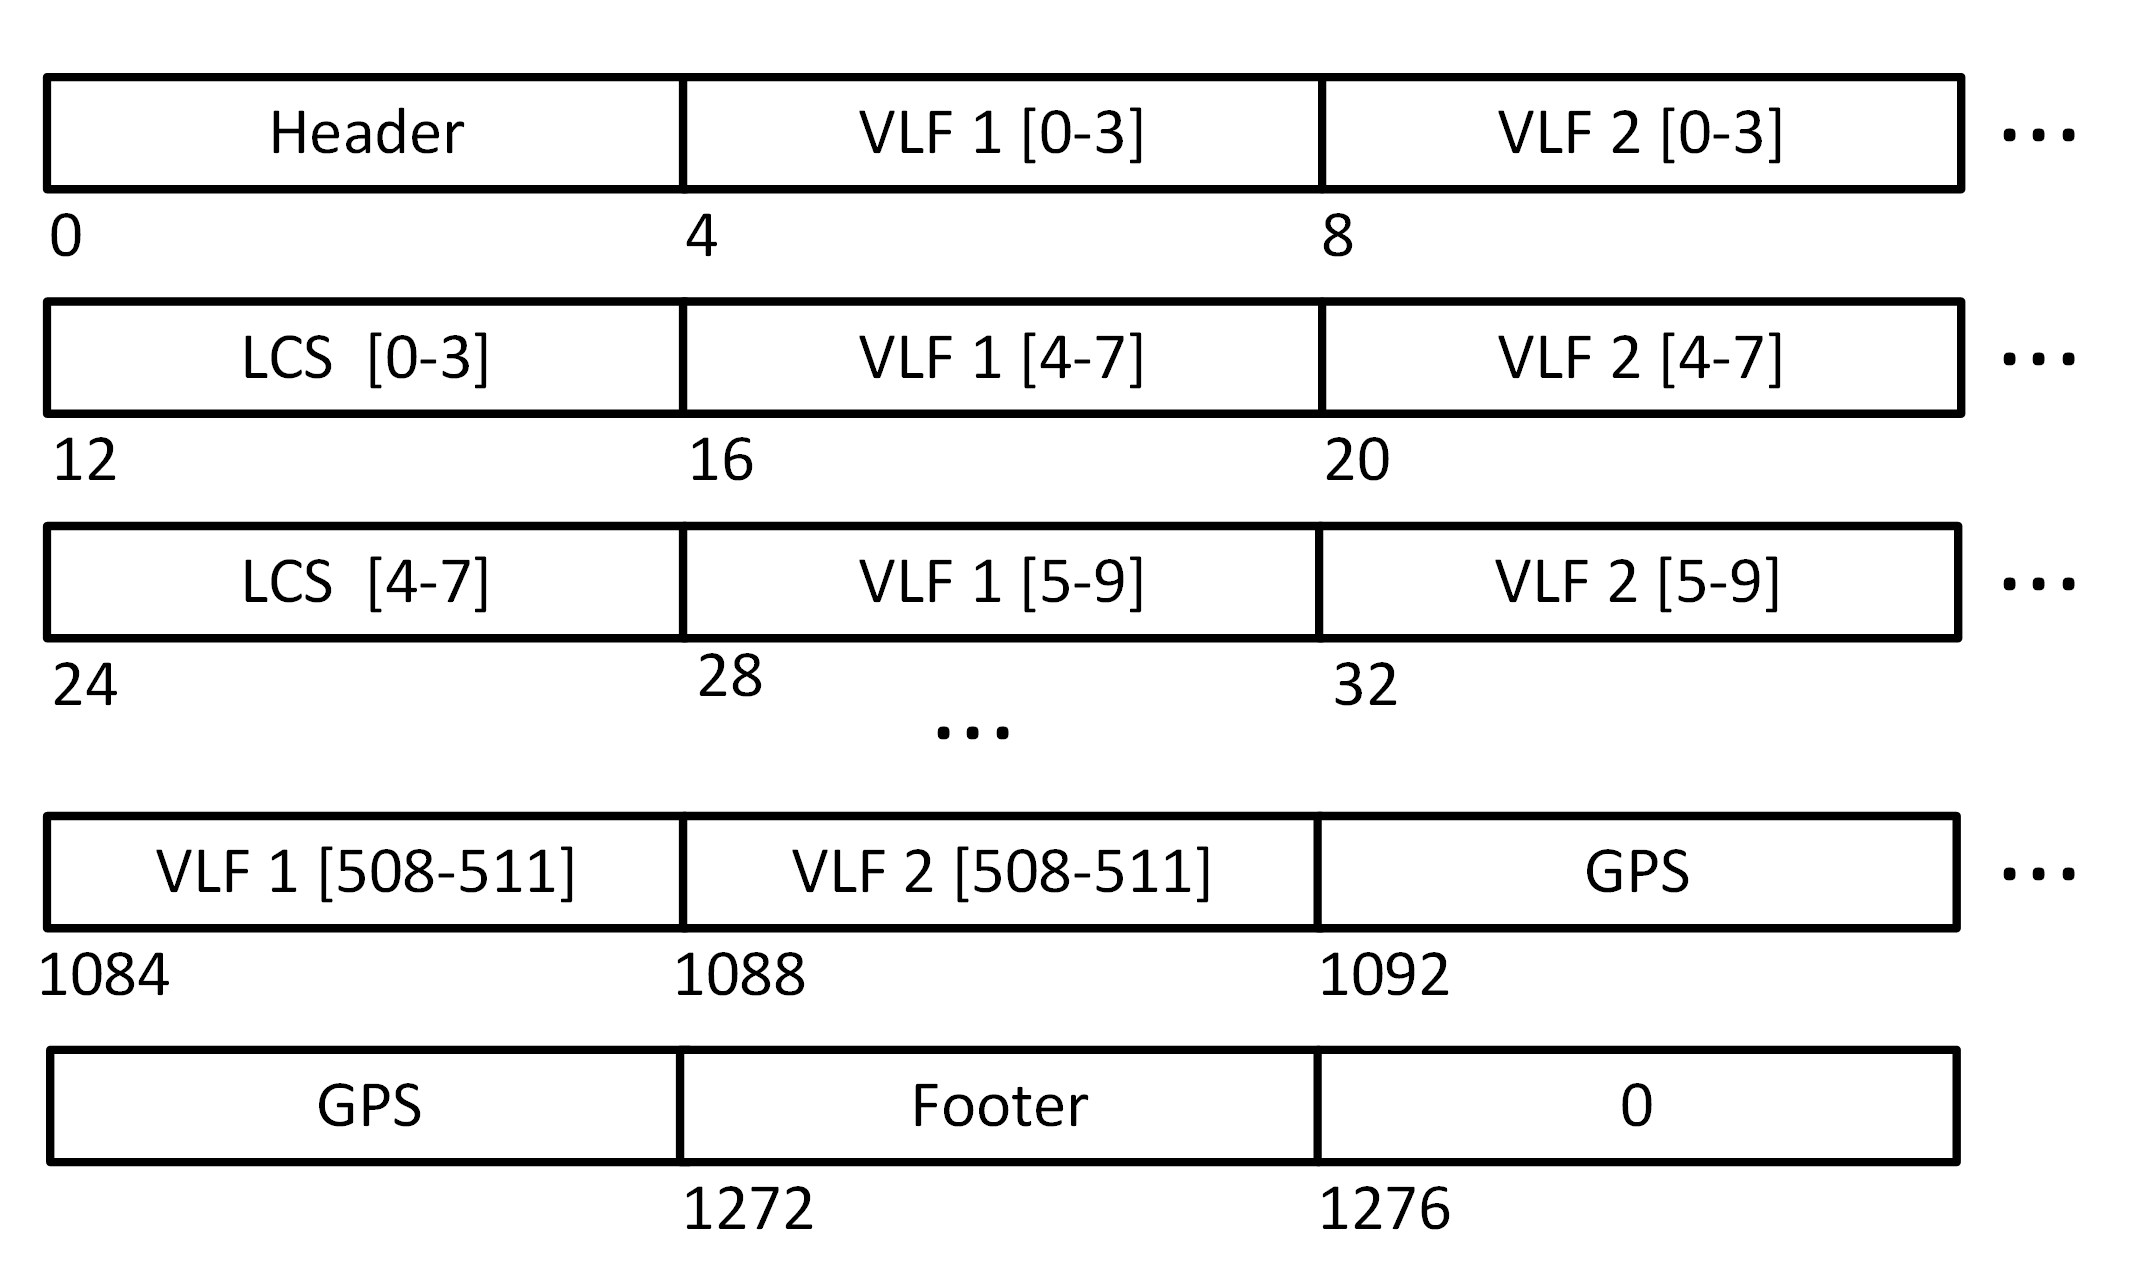
\includegraphics[width=20pc]{figures/vpm_figures/survey_datastructure_column_v2.png}

\caption[Interleaving scheme for survey data]{Interleaving scheme for survey data. A single survey column consists of 512 bytes from each of the two VLF channels, 64 bytes from the spectrometer, and 180 bytes from the GPS receiver. The data are interleaved in four-byte segments.}
\label{fig:survey_data_format}
\end{center}
\end{figure}
Each column of the survey product includes a complete GPS timestamp containing time, location, and velocity. GPS timestamps are collected every second; however no provisions are made to snap columns to the exact start time. Rather, survey columns are transmitted every 1024, 2048, or 4096 FFTs, depending on current configuration, with the GPS timestamp corresponding to the last whole second before the column is requested. In order to eliminate storage requirements for staging a survey column, data from the VLF receiver channels are interleaved, along with data from the particle spectrometers if present, into a 4-byte output stream.

Each column begins with a 4-byte header, 0xABCD-1234. Survey data is then presented four bytes at a time, alternating between the two VLF channels and spectrometer data when available. The data stream alternates between the two VLF channels when the spectrometer data has been fully read out. When available, the survey data is followed by a 180-byte GPS timestamp. Each survey column ends with a four-byte footer, 0x6789-1234, and an appropriate number of zeroes to assure a complete 32-bit word is passed to the memory controller. When both GPS and spectrometer data are present, the resulting column is 1280 bytes. The data format is illustrated in figure \ref{fig:survey_data_format}.

%Each column begins with a 4-byte header, 0xABCD-1234, followed by a 180-byte GPS timestamp (omitted when GPS timestamps are not available). Survey data is then presented four bytes at a time, alternating between the two VLF channels and spectrometer data when available. The data stream alternates between the two VLF channels when the spectrometer data has been fully read out. Each survey column ends with a four-byte footer, 0x6789-1234. When both GPS and spectrometer data are present the resulting column is 1260 bytes. The data format is illustrated in figure \ref{fig:survey_data_format}.



\subsection{Full-Resolution Burst Data}

VPM can log full-resolution data in a variety of modes, here referred to as \emph{experiments}. Data can be logged in either time or frequency domain, and can be taken on a modulated duty cycle, ranging from a single 30-second segment, to a selectable 1, 2, 5, or 10 seconds of data followed by a 2, 5, 10, or 30 second pause. The requested modulation will be repeated $nPulses$ times, which can be assigned via a separate command. When a GPS timestamp is available, an experiment will start at the next whole second after the burst command is received; if GPS card is not available, logging will start as soon as the command is received. Each subsequent on / off segment is tagged with a new GPS timestamp. A system status packet is logged at the beginning and end of each experiment.

Time-domain experiments can be taken at their full 80 kHz sampling rate, or decimated by factors 2, 4, 8, or 16. When decimation is selected, data is filtered using a 105th-order FIR low-pass filter. Filter coefficients were designed using the MATLAB Filter Design Toolbox (\emph{fdatool}), using the Least-Squares design algorithm. Cutoff frequencies were selected such that signals above the Nyquist frequency are attenuated by at least 60 dB. Filter coefficients are hard-coded and stored in on-chip ROM; filter delay lines are stored in on-chip RAM. Multiply-accumulate processing is done serially using a single hardware multiplier per channel. 

Maximum possible filter lengths are constrained both by available system resources, and by data sampling rate -- that is for each new data sample, we require $n$ multiplications. Given VPM's 10 MHz system clock and 80 kHz sample rate, a maximum filter is $\approx \frac{10e6}{80e3} = 125 $. $n=105$ was chosen to give sufficient padding for possible clock drift.

Frequency-domain experiments can be used to effectively reduce storage and transmission requirements in the event that only a small frequency band is of interest. The frequency range -- 512 bins, spaced uniformly between 0 and 40 kHz -- is split into 16 bands, which can be selectively enabled with each experiment. VPM uses two parallel FFT engines, which implement a 1024-point FFT, using a 50\% overlap and a Chebyshev window function with 75 dB sidelobe attenuation. Frequency data is accurate to a MATLAB or similar floating-point FFT computation to within 16 bits. 

Burst experiments are selected using a 24-bit command structure as shown in figure \ref{fig:burst_commands}. Each burst command begins with a header 2'b01. Bit three selects time-domain (1) or frequency-domain (0) data collection. Bit four enables time-axis duty-cycle modulation (``windowing"); bits 5 through 8 select the windowing pattern as shown in table \ref{tab:windowing}. For time-domain experiments, bit 9 enables downsampling and decimation. The downsampling factor is set by bits 10 and 11 -- 2'b00, 2'b01, 2'b10, and 2'b11 corresponding to 40 kHz, 20 kHz, 10 kHz and 5 kHz sampling rates respectively. For time-domain experiments, the remaining 13 bits are ignored. For frequency-domain experiments, bits 9 through 24 enable storage of each frequency band, from highest-frequency to lowest-frequency. Each band contains 32 FFT bins for a bandwidth of 2500 Hz.


\begin{table}
\centering
\caption[Burst mode duty cycle modulation settings]{Burst-mode duty-cycle modulation settings. Modes are listed as seconds on / seconds off.}
\label{tab:windowing}
\centering
\begin{tabular}{c|ccc|ccc|ccc|cc}
 0 & 10/30 & & 4 & 5/30 & & 8 & 2/30 & & 12 & 1/30  \\
 1 & 10/10 & & 5 & 5/10 & & 9 & 2/10 & & 13 & 1/10  \\
 2 & 10/5   & & 6 & 5/5   & & 10  & 2/5   & &  14 &1/5  \\
 3 & 10/2   & & 7 & 5/2   & & 11 & 2/2   & &  15 & 1/2  \\
\end{tabular}
\end{table}


\begin{figure}[t]
\begin{center}
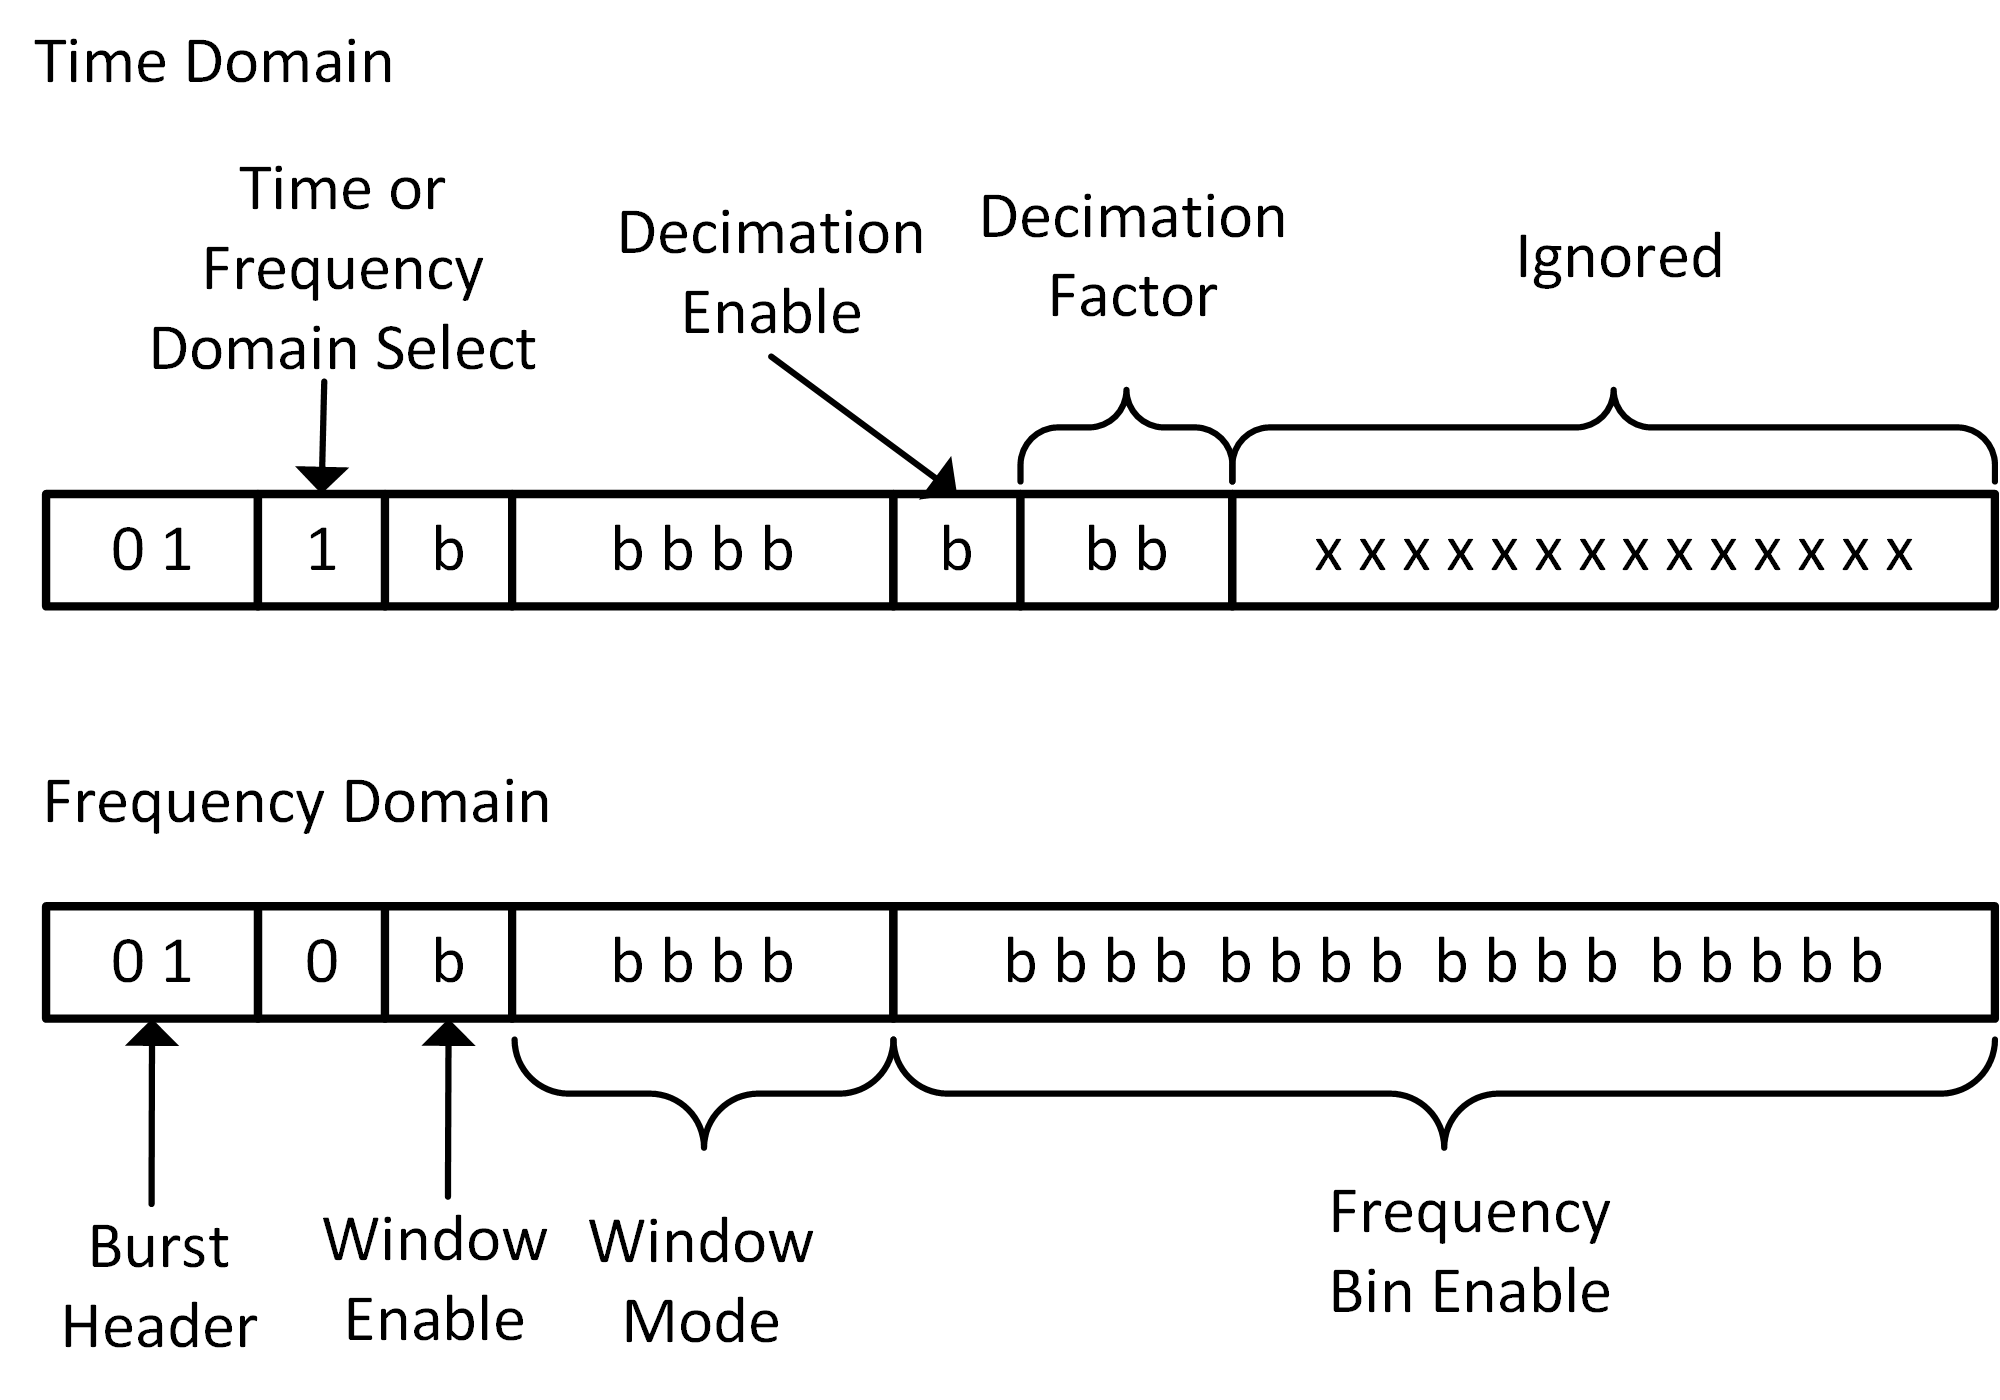
\includegraphics[width=20pc]{figures/vpm_figures/burst_commands.png}

\caption[24-bit command structure for burst experiments]{24-bit command structure used to request burst experiments. The top row shows a time-domain experiment; the bottom shows a frequency domain experiment.}
\label{fig:burst_commands}
\end{center}
\end{figure}


\subsection{GPS Timestamps}
VPM uses a NovAtel OEM 615 embedded GPS receiver which communicates directly with the DPU via RS232. When the system is reset, or when GPS synchronization is selected, the DPU requests two data products -- BESTPOSB and BESTVALB -- which provide solutions for position and velocity, encoded in a binary stream as described in \citep{novatel}. Timestamps are updated every second, and are accurate to the system sampling clock / PPS to $\pm 50$ ns. Together, the two data products occupy 180 bytes, and include position, velocity, and several metrics of quality-of-fit. Decoding can be done using the NovAtel Convert4 application, or our provided MATLAB script.

Figure \ref{fig:example_data} shows an example of a frequency-domain experiment, which has been windowed on both the time and frequency axes, and its corresponding survey data.

\begin{figure}[t]
\begin{center}
%\includegraphics{Figures/burst_example.eps}
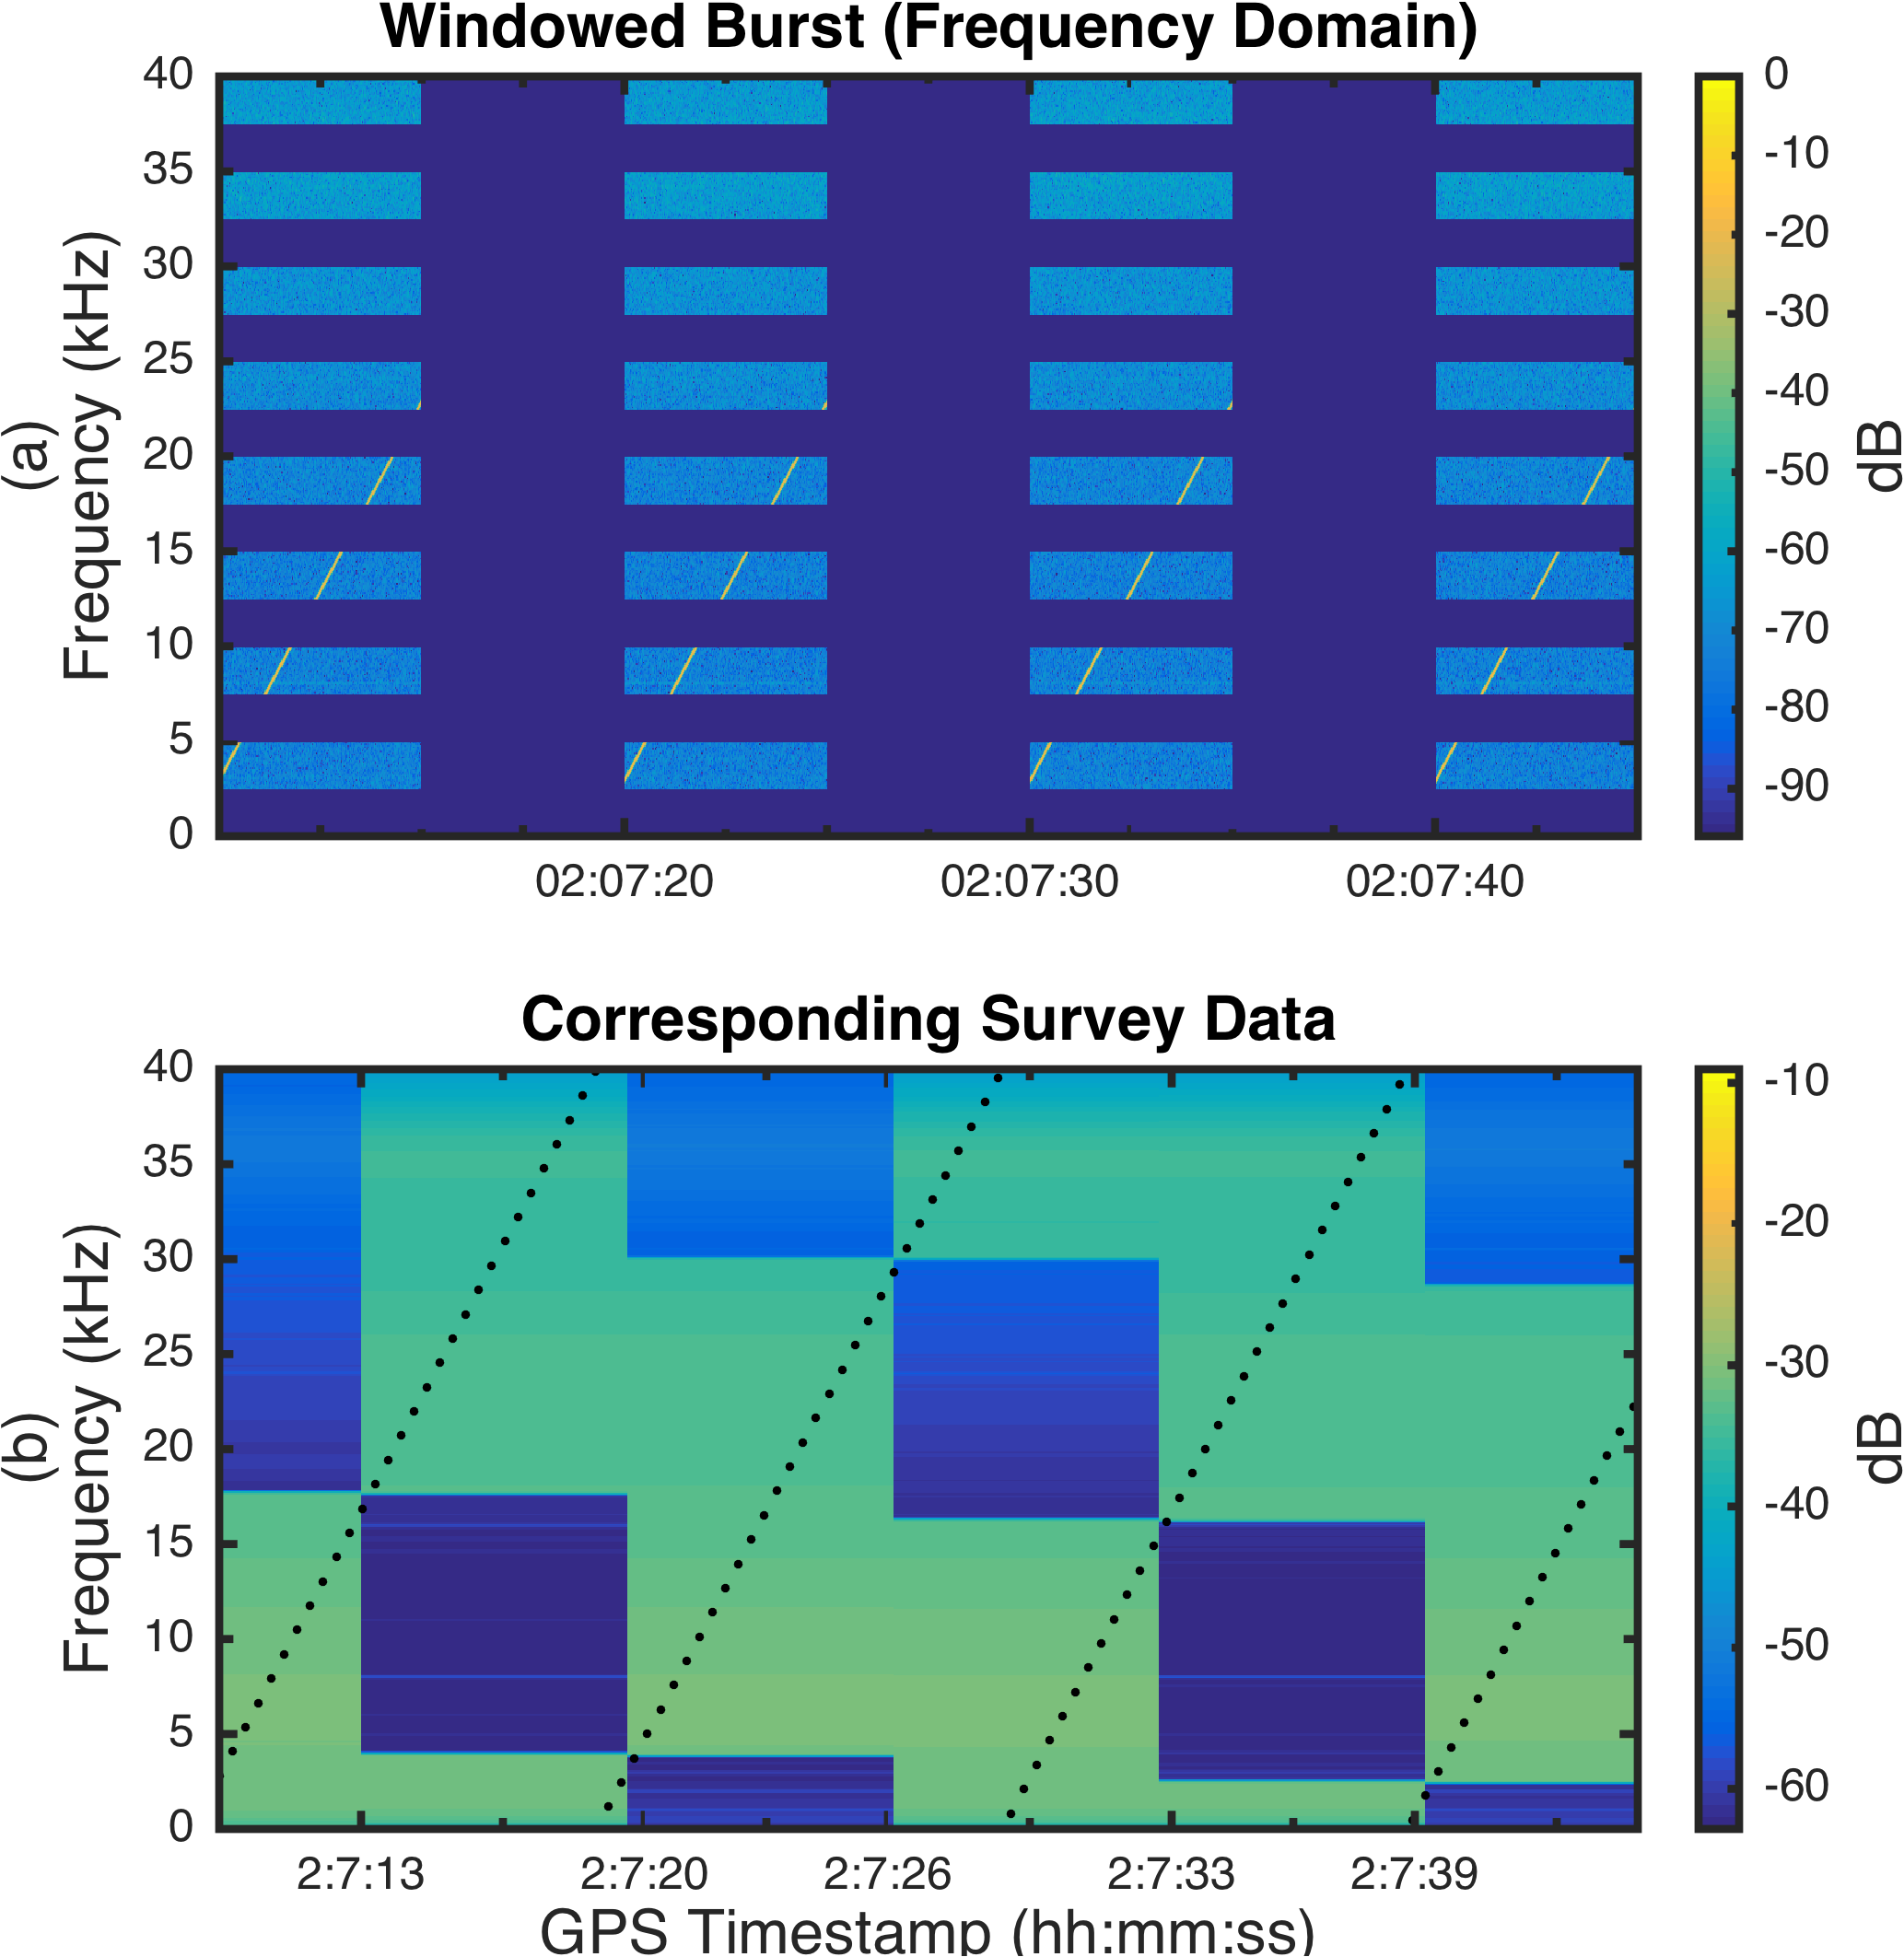
\includegraphics[width=20pc]{figures/vpm_figures/burst_example.png}
\caption[Example of a frequency-domain burst experiment and corresponding survey data]{An example of a burst experiment. Plot (a) shows the data returned from a frequency-domain burst experiment, which has been windowed in time using mode 6 -- five seconds on, five seconds off. Only every other frequency bin has been enabled. Input to the $\mu$BBR is a 10-second frequency sweep. Plot (b) shows the corresponding survey data, using the highest-resolution setting ($\approx$ 6.5-second bins). The dashed black overlay shows the approximate input frequency. Amplitudes are shown in decibels relative to full-scale.}
\label{fig:example_data}
\end{center}
\end{figure}


\subsection{System Status Messages}
VPM includes provisions for a single, comprehensive system status message. A system status message is logged at the beginning and end of each burst experiment; at the beginning of an antenna arm or deploy command; if the GPS receiver times out; or upon request by the host spacecraft.

Status messages include the following information:
\begin{itemize}
\item Source of the status request
\item Last command received by the system
\item System uptime in seconds
\item Total commands received by the system
\item Channel enabled / disabled status of E, B, and LCS burst data
\item Sampling clock selection - either GPS or internal
\item Deployer arm status for each antenna
\item Total attempted antenna deploys since last reset
\item Analog housekeeping mux setting
\item Survey product duration
\item Current burst repeat setting
\item Total packets sent from each data stream
\item Total bytes currently stored in memory
\item Current experiment number for each data stream
\item Total count of GPS errors and attempted resets
\end{itemize}
\subsection{Memory and Data Storage}
VPM lacks a full-fledged CPU and operating system, which necessitates the creation of a simple data handling and arbitration scheme. Use of a file system is avoided by regarding pre-transmission memory as a single buffering queue, with the expectation that data is read by the host spacecraft at the soonest availability. Memory management is divided into a set of packetizing modules -- one for each unique datastream -- which feed a simple arbitrating state machine. Complete packets are then stored contiguously in the external 128 MB SDRAM in the order in which they are generated. Packets are read contiguously, first-in-first-out. 

\subsubsection{Packeting}
VPM has facilities for six unique datastreams: Survey data; two channels of VLF data; spectrometer (LCS) data; GPS timestamps; and system status messages. Each datastream feeds an identical parallel packeting module, which writes packet headers and footers, logs metadata required in decoding, escapes header bytes from within the datastream, and inserts padding zeros to guarantee a consistent 512-byte packet. Packeting modules can each buffer two full packets before being read out.

Header and footer bytes are both 0x7E; however bytes in the datastream can take on all possible values between 0x00 and 0xFF. To prevent confusion when reading packets, we escape all instances of 0x7E within the datastream and insert a two-byte sequence 0x7D7D. Additionally, instances of 0x7D are replaced with 0x7D5D. To guarantee realtime streaming, escaping and external SDRAM reads and writes operate on a full-speed 20 MHz clock. 

VPM's packet structure is shown in figure \ref{fig:datastructure}. The following metadata are included in each packet:
\begin{itemize}
\item Packet Start Index (4 bytes): A four-byte integer representing the sample index of the first value within the packet -- used in assembling many thousands of packets from a burst experiment into a contiguous field.
\item Data Type (1 byte): Each channel is tagged with a single-byte label, denoting the packet's source: ASCII ``S" for Survey; ``E" for VLF 1; ``B" for VLF 2; ``L" for spectrometer data; ``G" for GPS data; and ``I" for system information / status messages.
\item Experiment Number (1 byte): Each experiment or survey column share a common experiment number, used to distinguish packets from sequential experiments.
\item Checksum (1 byte): A simple checksum is provided as a quick verification of packet health. VPM's checksum is a simple, 1-byte rolling sum of all prior bytes in the packet, including headers and escape characters. Two bytes are reserved in the packet order so that, in the event that the checksum value is escaped, the packet will remain a fixed size.

\item Byte Count (2 bytes): An integer representing the number of bytes contained within the packet, post-escaping. In order to maintain a fixed-size packet, data fields are padded with a variable number of zeroes. Three bytes are reserved for Byte Count in the event that the value is escaped. Note that only one value need be reserved, as the most-significant byte will never be escaped.
\end{itemize}

\begin{figure}[t]
\begin{center}
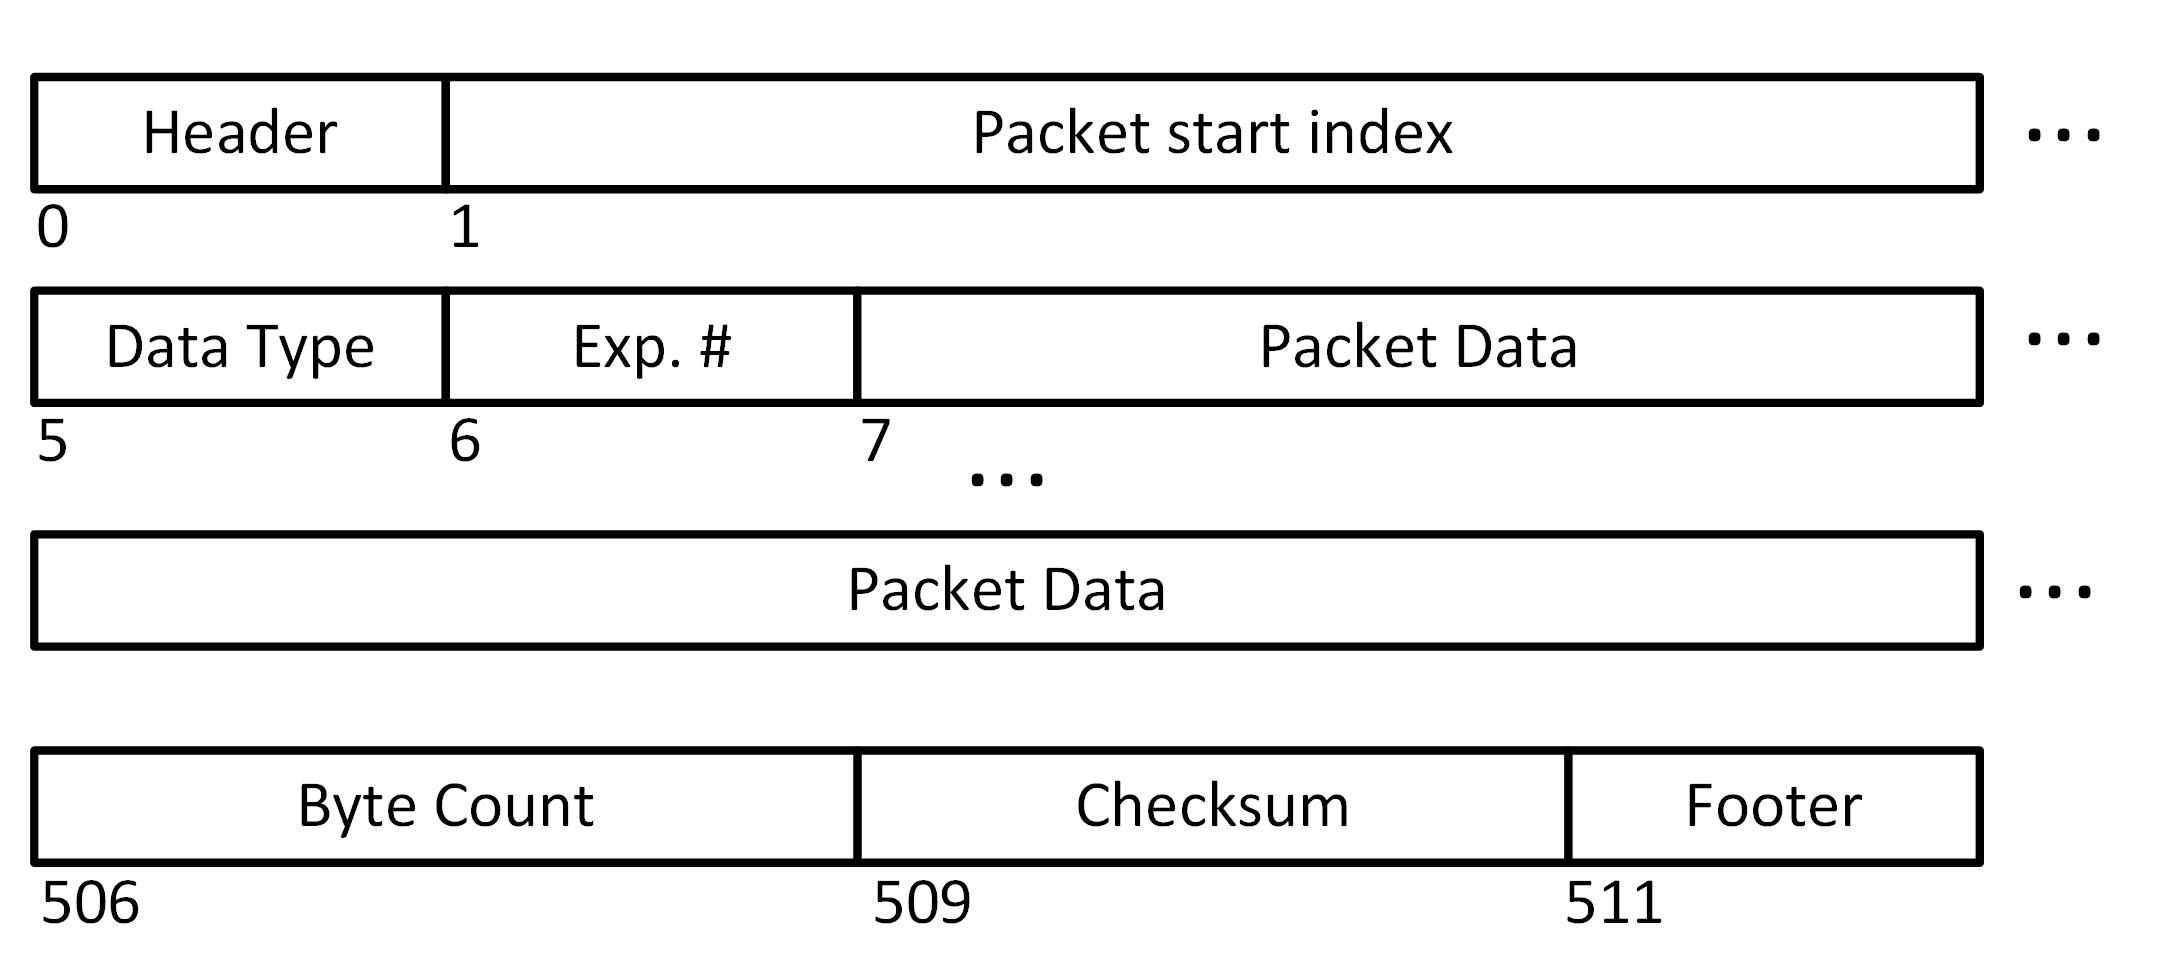
\includegraphics[width=20pc]{figures/vpm_figures/packet_structure_column.png}

\caption[Structure of packets returned by VPM]{Structure of packets returned by VPM. Packets include various metadata required for reassembly, and are zero-padded to assure a constant size of 512 bytes.}
\label{fig:datastructure}
\end{center}
\end{figure}

\subsection{System Control}
Commands are passed to VPM through the RS422 port, which operates at 400 kilobaud. Commands are received by a simple format-checking state machine. All commands are 24-bit, and of the form: $\{$ 0x7E $\|$ Byte 1 $\|$ Byte 2 $\|$ Byte 3 $\|$ 0x7E$\}$. Bytes are reassembled in big-endian order. Commands which do not meet this form exactly are discarded; however, the three command bytes must be escaped in the same manner as on transmission if they include a 0x7E or 0x7D value.

Successfully-received commands are passed to a master state machine, which then sets global parameters and passes commands to submodules accordingly.

The first two bits of a command dictate the intended recipient: 2b'00 for DPU and system commands; 2b'01 for burst commands; 2b'10 for $\mu$BBR commands; and 2b'11 for commands sent to the loss-cone spectrometer.

DPU commands are in a human-readable ASCII character format (``G1" = Enable GPS, ``G0" = Disable GPS, etc). Burst and $\mu$BBR commands assign a specific purpose to each of the remaining 22 bits.


\section{Concluding Remarks}
We have described a novel design for a CubeSat payload instrument, which is capable of sampling the VLF band of the electromagnetic spectrum while simultaneously sampling energetic particle distributions of the radiation belt. The system draws less than 5 Watts including the onboard GPS receiver, and occupies a 1.5U volume. The system provides two data products -- a low-resolution survey product which runs continuously, and a full-resolution burst product, which is available on demand from the host spacecraft. The onboard software is implemented entirely in an FPGA fabric, eliminating the need for additional volatile program storage, which reduces risk of CPU errors and improves system reliability. Additionally the system can be implemented using radiation-tolerant components. A CubeSat carrying the VPM payload is scheduled to be launched by the Air Force Research Laboratory in 2019.



